%\documentclass[man]{apa}
%\documentclass[doc]{article}{styles/apacls/apa}
%\documentclass{report}
%\documentclass[man]{styles/apacls/apa}

%\documentclass[11pt,twoside,a4paper]{article}
%\documentclass[11pt,twoside,a4paper]{book}
%\documentclass[11pt,twoside,a4paper,openright]{report}
\documentclass[11pt,oneside,a4paper,openright]{report}

\usepackage{mathptmx}       % selects Times Roman as basic font
\usepackage{helvet}         % selects Helvetica as sans-serif font
\usepackage{courier}        % selects Courier as typewriter font
\usepackage{type1cm}        % activate if the above 3 fonts are
                            % not available on your system
\usepackage[utf8]{inputenc}
\usepackage{textcomp}
\usepackage{makeidx}         % allows index generation
\usepackage{graphicx}        % standard LaTeX graphics tool
                             % when including figure files
\usepackage{multicol}        % used for the two-column index
\usepackage[bottom]{footmisc}% places footnotes at page bottom

\usepackage{verbatim}        % per comentaris multilinia
\usepackage[utf8]{inputenc} %permite escribir {\'a},{\'e},{\'u},{\'o},{\'\i} & {\~n} directamente
\usepackage[british]{babel}
\usepackage{csquotes}
\usepackage{amsmath, amsthm, amssymb}
\usepackage{enumerate}
\usepackage{algorithm2e}
\usepackage{pdfcomment}
%\usepackage[lined,boxed,commentsnumbered]{algorithm2e}


\begin{document}
\newpage

%\textwidth 6in \oddsidemargin 0.2in \evensidemargin -0.2in
%\textheight 9in \topmargin -0.75in \headheight 0mm \headsep 25mm

%\Large
%\addtolength{\hoffset}{-2cm}

\pagenumbering{roman}

\newpage 

\setcounter{tocdepth}{6}
\tableofcontents
\newpage 

\pagenumbering{arabic}

	
\chapter{Model-0 Experiments}

The chapter of experimental results follows part of the trajectory of the experience of comparing the 
performance of the AI agents versus the classical rule agents. The first results are related to the first
experiments of rule based agents in the model for the Gujarat\cite{JARM2014}. Taking the same setting, 
mdp agents were put to test showing us that they could not improve the rule based agent resilience capability.  
The multiplicity reduction of the planning search states(p.\pageref{sec:ReduccStates}), compacting the range of values and 
limiting stochasticity, proved to be a good solution to solve it. Results are shown where it is obvious that 
starvation is lower for mdp agents. Afterwards, some odd trends in the behaviour of parameters of the decision 
making process motivated another analysis of the model for the knowledge layer of the agent 
(p.\pageref{sec:Divergence}). 
Managing the change of biomass due to biological growth and decline of resources is introduced in the mdp 
layer of the agent. Following, results showed that tackling with resource grow/decline prediction contributes 
with only a slightly upgrade of starvation rates. Next experiment tries to set a lower bound to starvation 
rate based from biomass guessing and optimality of resource retrieval(p.\pageref{sec:NoDepletionExperiment}). The breach, 
that marks the distance to the ideal foraging, seems only to be explained by uncertainty an stochasticity 
effects, and not a big advance can we get from refining further the biomass prediction procedures. Many of 
these experiments are run under an scenario where the agent is alone in the world. One of the motivations is 
to discover faults in the foraging and migration patterns and verify the modeling decisions.
That is the reason that introducing divergence management due to neighbour presence (multi-agency) is left 
for the next step of this model in the project. But anyway, although there is no multi-agency awareness we 
have tested the agent in a scenario of indirect competition for resources with other agents.

Three more packs of experiments follow to complete the chapter now focused on the differences between AI 
agents and classical simple agents. First there is a straightforward comparison of annual starvation rates
between the random agent, the rule based one and several configurations of mdp agent. The next experiment
is the extended version to a ten year trace. And finally there is an exploration of the relevance of adding 
more iterations to the deliberative engine of the agent. We observe a consistent advantage of the mdp agent
over the rule based agent. We will expose the evidence in the numbers and also in the patterns of mobility 
produced by the logic of the rules. Following the trace of actions and change rate in starvation we could 
glimpse that the mistakes of the rule based agent were directly related to a problem of inability to adapt 
to two time lapses in the year were opposite strategies were needed.


\section{Tunning the planner ( State Reduction And Statistical Significance )}
\label{sec:expStateReduction}

%%quick descrip : 
This section exposes the first results and issues of the tests of the mdp agent under the same conditions 
that the rule based agent was run\cite{JARM2014}. An Agent Based Model(ABM) of rule based agents was designed to study 
resilience and persistence of Hunter-Gatherers(HG) in the north zone of Gujarat, a north-east province in India. 
The topic question was rooted in the premise that the main factors conditioning the presence of HG were 
related to climatic changing conditions and its effect on resource availability. 
Simulations were run taking the climatic conditions of three spatial bounds, the zone of Kutch-Saurashtra 
(north Gujarat), the region of Gujarat and the average rainfall of the whole continent. The combination of
the regions, the extrapolation of climatic parameters to four selected time lapses in Holocene plus the 
intervals of exploration of the rainfall ( average and yearly variation ) unfold the simulation scenarios.
The analysis shows that historical decrease of average rainfall along millennia is not enough explanation 
to answer the question about extinction of HG. On the other hand, variation associated to yearly precipitation
played a strong role on population dynamics as the major cause for group collapse if a threshold is 
surpassed. Although, the conclusion is open to consider feasible that other factors coocurred with rainfall 
variation in the decline of the HGs.

Against our intuitions the mdp agent could not break the starvation rate of the rule based agent. Statistical 
sampling of the starvation rates showed us a performance equivalent to the rule based agent. Furthermore, 
the exploration of different parameters in the planning engine did not produce improvement and results were unstable. 
We saw agents with deeper future prospection and greater sampling in the search tree to perform sometimes 
worse than other configurations.

%%describe plots : 

Fig.~\ref{fig:noReduccClim4000} is a sample simulation of one year run illustrating the performance of mdp 
agents versus the rule based agent in the scenarios from the above paragraph. Agents able to prospect three 
days in advance were not able to surpass the one day time frame of the rule based agent, and agents with a 
horizon of six days got only a small advantage compared to our expectations.

\begin{figure}[!htb]
\centering
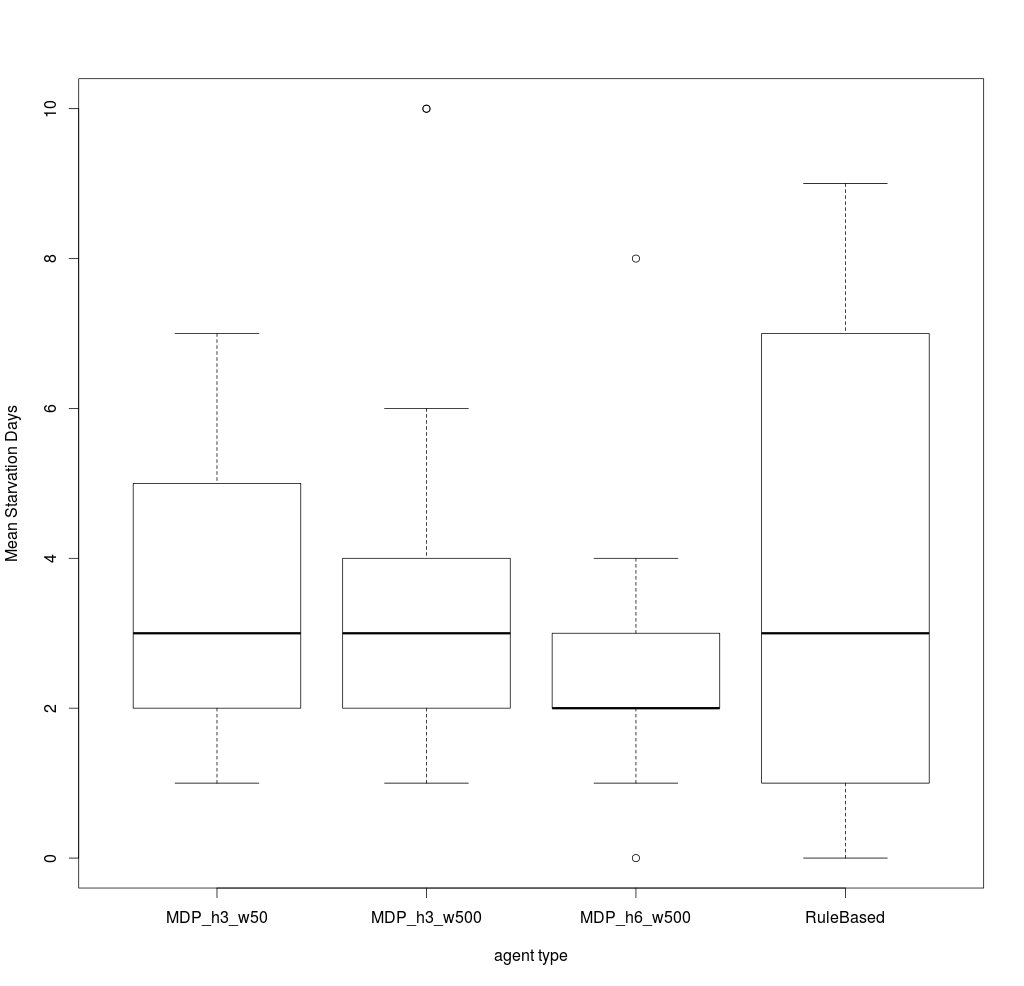
\includegraphics[height=12.2cm]{figures/expm/noReduccClim4000}
\caption{Comparing Rule Based Agent with MDP agents under North Gujarat rain condition, 4000 rainfall 
units/year.}
\label{fig:noReduccClim4000}
\end{figure}

%%brief conclussion:  

The problem lied in the internal representation of the world for the search nodes of the mdp layer. The 
representation scattered the states due to the wide domain of the features. It produced non matching states
and led to search traces with low statistical significance needed to distinguish preferable traces
from the harmful ones for the agent. The representation of the world states was reduced categorizing numerical
features and reducing stochasticity the children node states expansion as the corresponding section illustrates
(p. \pageref{sec:ReduccStates}).
After state reduction the results took the direction we were expecting. The figure 
~\ref{fig:meanBoxplots_Rain1000to4000_rule_rand_mdp} corresponds to an exploration of the rainfall in the 
interval from a quarter of the mean to the mean of rainfall in KS-Gujarat scenario. For each value of rainfall
in the axis there are ten runs with an associated starvation rate distribution as output measure. For
each set of runs we register the mean of starvation rate and represent it in the plot with coordinates the 
rainfall and starvation rate involved. Each of the dots is connected with lines to its adjacent neighbours 
to reveal visually the functional relationship between the variables. 
The shape exposes an exponential growth of starvation as agents are deprived of resources due to scarcity of 
rainfall. For the mdp agent the slope is not so high and the proportion is quite a few times lower than the 
rule based agent. Also the shape of the starvation along the axis is far less bumpy, meaning that the response 
of the agent is more uniform and stable. Less variation in getting the resources means robustness to change
and hence we can see it as a clue of greater adaptability.

\begin{figure}[!htb]
\centering
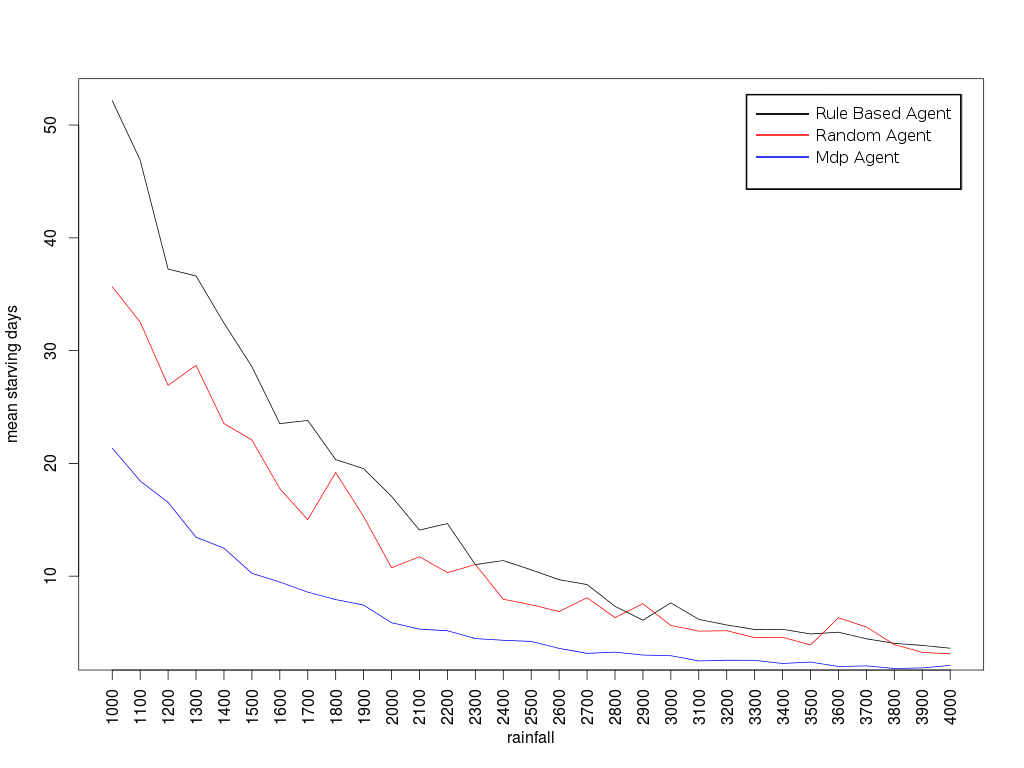
\includegraphics[height=12.2cm]{figures/expm/meanBoxplots_Rain1000to4000_rule_rand_mdp}
\caption{}
\label{fig:meanBoxplots_Rain1000to4000_rule_rand_mdp}
\end{figure}

The plot shows an extra agent labeled as Random. This agent chooses an action with uniform and equal 
probability from the combination of the actions and sectors where the action can be applied. This agent 
was introduced to have its performance as reference in the comparisons. 

Below, you can find a detailed explanation of the results discovered for the rule based agent and why they 
are worse(p.\pageref{sec:expEcsi1}).
The enumerated reasons are related to the cause why we have the unexpected result of the random agent's 
performance being better than the rule based one. The conditions of movement of the rule based agent polarize
in two results tied to the two critical moments of the year, the beginning and the end. 
For one case, the agent launches more movement actions than what is advisable; for the other case, the agent
delays too much the next move action to launch. The random agent with its uniform distribution of actions does 
not replicate the same movement patterns that harm the rule based agent avoiding the penalties in starvation.

\section{Divergence And Biomass Prediction}

%%quick descrip : 

Having managed to offer a better response than before (Fig.~\ref{fig:meanBoxplots_Rain1000to4000_rule_rand_mdp}), 
the next step was to explore the best parameters for the simulation with mdp and find a lower bound to the 
achievable starvation or a feasible balance between depth of reasoning and CPU time.

Our simulations explored the parameter horizon and width of the UCT algorithm\cite{BonetGeffner2012}. The expected 
result was to find how starvation decreased as we increased horizon and width in parallel. We did not paired
low values of width to the higher values of horizon of the exploration set. UCT follows a search tree of 
states where depth is the horizon parameter and width the amount of traces that are launched against the tree 
to retrieve a sample of its leaves to produce a eligible set of future desirable states. Horizon values in
exploration must grow paired with width. Low values of width retrieve poor samples from a huge pool of leaves 
if horizon is big enough. 

%%Settings : 
%%describe plots :

One part of the simulations helped to discover that for higher values of width and horizon we got no 
improvement in resilience in comparison to other runs with lower horizon. Also, for a same horizon, greater
width had a negative impact on starvation rates(Fig.~\ref{fig:widthsNonMonotonic}).

%observacio/evidencia:
%ecsi3 -> diferents widths, veus widths mes alts que haurien de millorar l'starv i no,
%ho fan pitjor que d'altres -> mostrejant estats incorrectes generats per la divergencia

\begin{figure}[!htb]
\centering
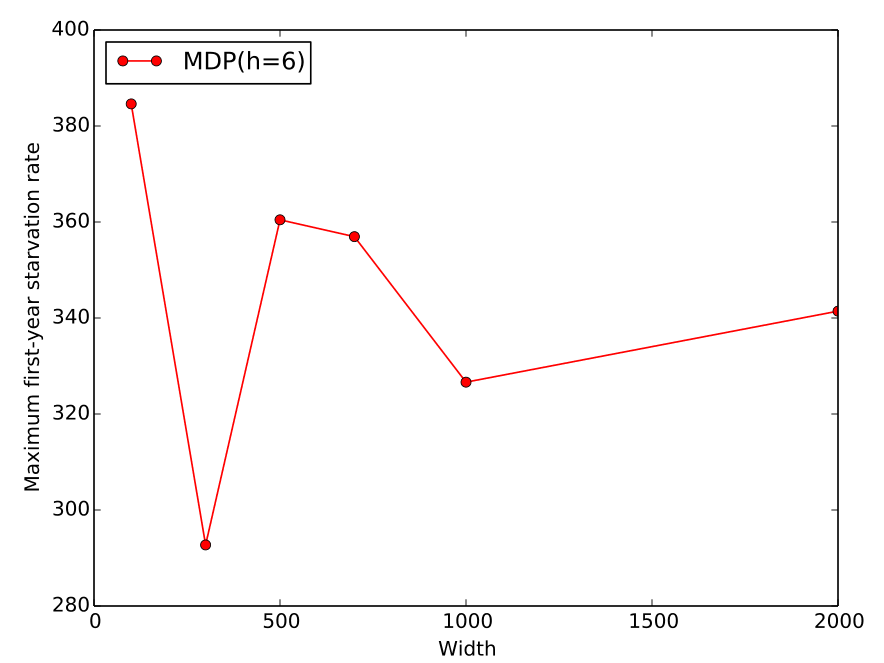
\includegraphics[height=8.2cm]{figures/expm/widths}
\caption{Exploration of width parameter showing non monotonicity.}
\label{fig:widthsNonMonotonic}
\end{figure}

%%brief conclussion:
The same happens in weather forecast. As we put farther the day we want to know its weather, the worse is
the prediction. Weather simulation works over a representation of the world. There are not perfect measures,
all the variables are not taken into account to design the model and at the end, they sum up in the 
accumulated error, step after step of the simulation. This leads to a state which is different to the one 
that will happen. We call this divergence of traces(p.\pageref{sec:Divergence}); divergence between the real trajectory and the simulated trajectory. Divergence happens because we introduce some error or because the model is incomplete; indeed, it is always incomplete.  
  

%%TODO move it to DivergenceModelChapter
%%BEGIN
UCT uses an internal model emulating the real world model in order to explore the choices that must offer 
to the agent. The model that UCT executes in this decision making process does not take into account two 
important points of the mechanics of the environment. First, each time-step, resources automatically grow or 
decrease depending on the season of the year; they do not remain constant. Second, the agent is not aware of 
any neighbour present in its home-range. 

UCT launches a path from the root node to one leave node generating a search tree on-the-fly. There will be 
as many shots as the amount assigned to the width parameter. Each step, from one parent node to a child node, 
is executed as a simulation over the structures that are the representation of the world inside the 
UCT process. If the dynamics do not apply growth or shrinkage of resource due to climate or resource depletion 
exerted by other agents, there will be incoherence. The state will register a false amount of resources.
The procedure will continue along the path towards the final leave node assigning deviated utilities to 
states that should have a different quantity of resource. An incorrect assignment of utilities in states
leads to misinformation in the search process, an a bad classification of the traces considered as a good
prediction of what will happen if the sequence of actions associated to the path is executed. Misinformation 
leads to divergence which will lead to loosing predictive power in the UCT. If you increase width you increase
the weight of diverging states because you are repeating the same faulty procedure time after time loading of
statistical weight to bad scored states. This way, width does not imply to be more informed. Increasing 
misinformation implies more uncertainty, and more bad choices for the agent.
%%END

%%TODO posa tot aixo al capitol del model del agent i referencia desde aqui
%\ref{DivergenceChapter}
%pq estudiem la divergencia
%sabem que els recursos fan una trajectoria triangular --> una mateixa quantitat de recurs 
%apareix 2 cops a l'any, al pujar i al baixar. Dos contextes diferents.
%Una manera de detectar aixo es que l'agent pugui saber en quin moment de l'any esta
%i llavors que pugui induir aquella quantitat esta en un contexte de pujada, o de baixada.
%L'altra manera es permetre-li predir el creixement/decreixement de biomassa, i aixi
%integrar tota la informacio... 
%Divergence And Biomass Prediction <-- cross ref

Experiments in this section test the benefit from adding biomass growth prediction to avoid divergence due 
to bad biomass estimation in the planning process. 
Equivalent scenarios were applied to search for a way to solve the phenomena announced above. 
The experiment tests one single agent for a year against three different rainfall conditions. The first
condition uses 500 rainfall units to set an environment that will ensure a noticeable amount of starvation 
rate. The next scenario has a rainfall of 1500 units to have an intermediate stage between the first and
the third which reproduces a mean rainfall similar to Gujarat, 4000 units.
%%plot description
The experiments register the starvation rate as an indicator of better performance of the agent that applies
biomass prediction. We have labeled the agents as Guessing and NoGuessing in the plot, the former 
corresponding to biomass prediction to avoid divergence, and the later corresponding to not applying biomass
growth prediction. For rainfall with 500 units, there are few resources and it is hard to mark a difference 
because there is no space to exhibit a big exploitation of the terrain 
(Fig.~\ref{fig:guessVSnoguess_clim500.png}). With rainfall 1500 the improvement is less than 1\% 
(Fig.~\ref{fig:guessVSnoguess_clim500.png}); and with 4000 units of rainfall the starvation falls only a 5\% 
of the value (Fig.~\ref{fig:guessVSnoguess_clim500.png}), from 1.55 to 1.475 as an average.
Is it possible to devise a way of taking more profit from biomass prediction? There is any fault in the way 
we applied prediction in the states of the planning procedure?
Next section discusses and reasons about the causes of the little effect of applying biomass prediction
in solving the biomass divergence. 

\begin{figure}[!htb]
\centering
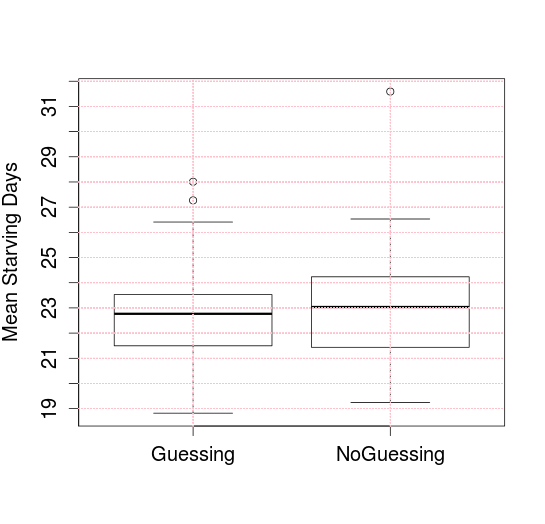
\includegraphics[height=8.2cm]{figures/expm/guessVSnoguess_clim500.png}
\caption{Mean Starvation days for an agent that predicts biomass grow and decrease versus
an agent that does not apply a grow/decrease factor during the decision making. Experiment 
run with 500 units of rainfall. }
\label{fig:guessVSnoguess_clim500.png}
\end{figure}

\begin{figure}[!htb]
\centering
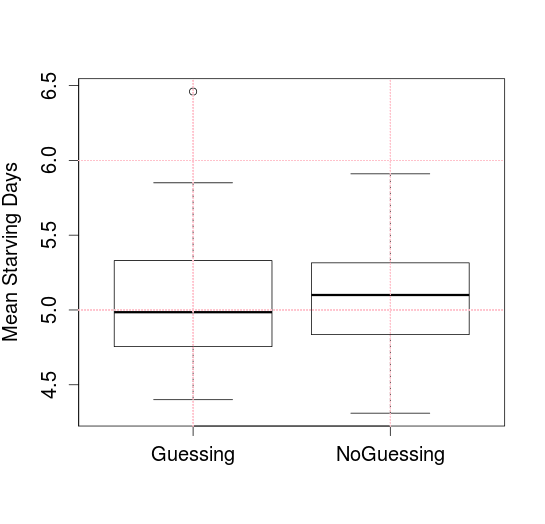
\includegraphics[height=8.2cm]{figures/expm/guessVSnoguess_clim1500.png}
\caption{Mean Starvation days for an agent that predicts biomass grow and decrease versus
an agent that does not apply a grow/decrease factor during the decision making. Experiment 
run with 1500 units of rainfall. }
\label{fig:guessVSnoguess_clim1500.png}
\end{figure}

\begin{figure}[!htb]
\centering
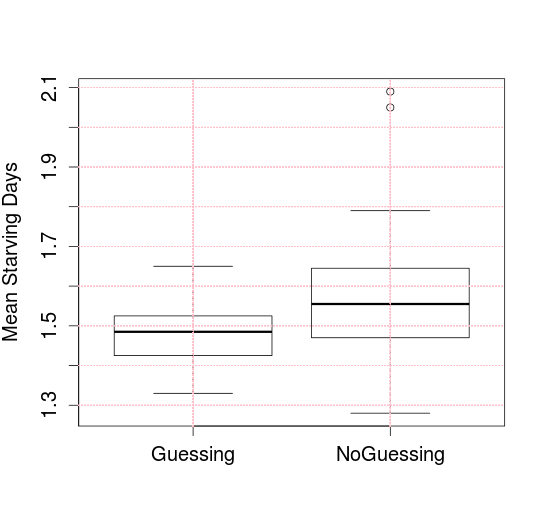
\includegraphics[height=8.2cm]{figures/expm/guessVSnoguess_clim4000.png}
\caption{Mean Starvation days for an agent that predicts biomass grow and decrease versus
an agent that does not apply a grow/decrease factor during the decision making. Experiment 
run with 4000 units of rainfall. }
\label{fig:guessVSnoguess_clim4000.png}
\end{figure}


\subsection{Finding the limits to Improvement by Biomass Prediction}
\label{sec:NoDepletionExperiment}

%%quick descrip : 

The results of the experiment in the previous section, contrary to the expected, do not show a substantial 
improvement when the agent predicts biomass when compared to the agent that does not use prediction. Clearly,
the depths of exploration we use, three, six, ten days forward, do not allow to accumulate an excessive 
divergence because there is not enough length in the trace. In particular, when the agent is at the 
end of the year, when the agent exhibits a greater movement rate, fewer days are spent camping in the same 
settlement. The resources in the location are perceived along a very short segment of time. And reasoning
about resources in a small window of time should not involve critical divergent traces. But on the other hand,
decline of biomass moves forward and it is logical to expect that without biomass-prediction the planning
process will suggest to move when it is too late and you will fall into the error of waiting too much in a
poor resource area. One of the two possibilities must be discarded. We could think that the procedure for 
predicting biomass is not sufficiently accurate or incorrectly focused. 

The experiment of this section was designed to assure ourselves about this matter. The target is to attempt 
to establish a lower bound to the starvation rate. We will see that there is a gap between the profile of 
an agent with biomass-guessing and the profile of the lower bound. The lower bound is given by a modified 
mdp agent whose foraging actions although return a reward, it does not deplete the resource patches. 
The experiment executes a normal mdp agent, a no-depletion agent and a modified simplified setting, let's call
it the ``gap agent''. The idea is that the simplifications allow to jump the gap of the difference between the 
starvation rates of the normal agent and the no-depletion agent. The intuition is that this modifications 
will be related to why the mdp agent cannot get nearer the lower bound. The modifications are detailed next. 
The normal agent receives normally distributed reward from the forage actions in the real world, and in the 
planning process. When a move action is launched the reward of the day is halved compared to a foraging 
day. The gap agent does not have stochasticity in rewards and receives full reward from foraging actions all 
days. This modifications are related to uncertainty in reward and uncertainty in appropriate election for a 
move action. Foraging actions without stochasticity produce better prediction of rewards in the planning part 
of the agent. Removing uncertainty and seeing that the starvation rate for the gap-agent matches the 
starvation rate of the no-depletion agent will tell us that the gap can be explained by uncertainty non 
related to biomass guessing and the divergence problem.

The way of producing the lower bound tracing the no-depletion agent has the following reasons. The track of 
the interaction of an agent with the world is a sequence of actions. Along the simulation, the agent produces 
a list of move and forage actions. Usually we will see sequences of forage actions between move actions 
denoting the pieces of time that a settlement occurs in a location till the next movement. The challenge 
for the planning layer is to propose movement actions in a way that the intermediate forage actions can 
always retrieve a maximal amount of resources. The ideal situation would be one were the foraging actions 
will endow the agent with enough resources to achieve the metabolic needs. And when no more foraging actions 
can be added to the sequence due to resource depletion, a move action must be launched to a new area plenty 
of resources. 

The day when a movement action is launched, the agent receives resources from a secondary forage action that 
is bonded to the movement action. The reward is half of a normal forage action that would be launched in a 
day where only forage happens. It is critical to choose the step to launch the movement and minimize the 
effect of receiving only half of the reward. It is the most demanding feature for the planner apart of moving 
the agent towards richer areas as a long term effect of the drift of the movement. The artificial ideal planner 
would be imagined free from bad allocated move actions. The artificial ideal planner is imagined as proposing 
always movement actions in the time step when they would not increase the starvation of the agent. So that is 
what happens when you do not apply the depletion of resources to the environment after the execution of a 
forage action. Because the resources stay unaltered as if the patch were new and the agent just would have 
arrived in the last time-step. And then it seems that the sequence of actions does not disturb the flow of 
resources that the agent retrieves. It seems as if the planner would have been selecting each time the perfect 
action to be launched; either a normal foraging action or a move action in the time step before the system reaches 
a state low in resources, when the half forage does not cover the survival threshold. 
Why do we not fill the environment with infinite resources, and then have forage actions returning always
plenty of resources? The infinite resources setting would not exhibit phenomena like the ideal planner in the 
original world model. There are seasons in the year, at the beginning and at the end, where biomass dynamics 
produce a low load of resources in the environment. Applying infinite resources masks this phenomena and also
would produce a too low lower bound. Doing no-depletion consists in reading the amount of resources, apply the 
foraging formula and give the result to the agent without updating the world. But this does not mask the 
effect of biomass dynamics. Because in the poor days of the year the formula of foraging returns low rewards.
At the beginning of the year there will be low resource because biomass has not fully grow and the end of the 
year there will be less resources because of the effect of biomass decline procedure. The most perfect planner 
would find this situation, and could not give to the agent a recommendation that would allow recover more 
resources than the low amounts present in the poor days of the year. The ideal planner conceptualization must 
not avoid the increase of starvation in these cases. It can manage to reduce it to a minimum but can not keep 
it to level zero for ever and for any condition. This discards the option of using infinite resources as a 
medium to produce a lower bound to starvation rates, and strengthen the use of no-depletion.

%%Settings : 

%%describe plots :

\begin{figure}[!htb]
\centering
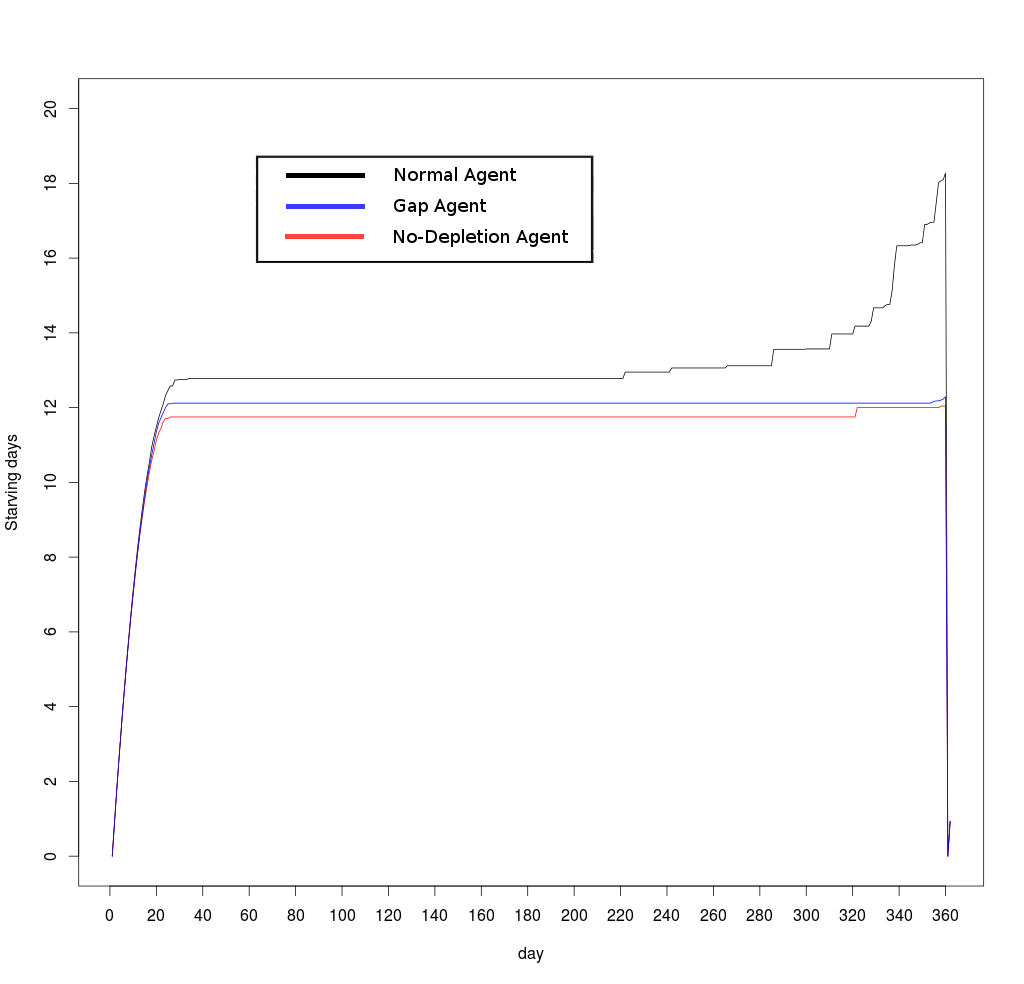
\includegraphics[height=12.2cm]{figures/expm/gapExplainClimate500}
\caption{Overlapped starvation profiles of the agents in the no-depletion experiment with a rainfall of 500 
rain units .}
\label{fig:gapExplainClimate500}
\end{figure}


\begin{figure}[!htb]
\centering
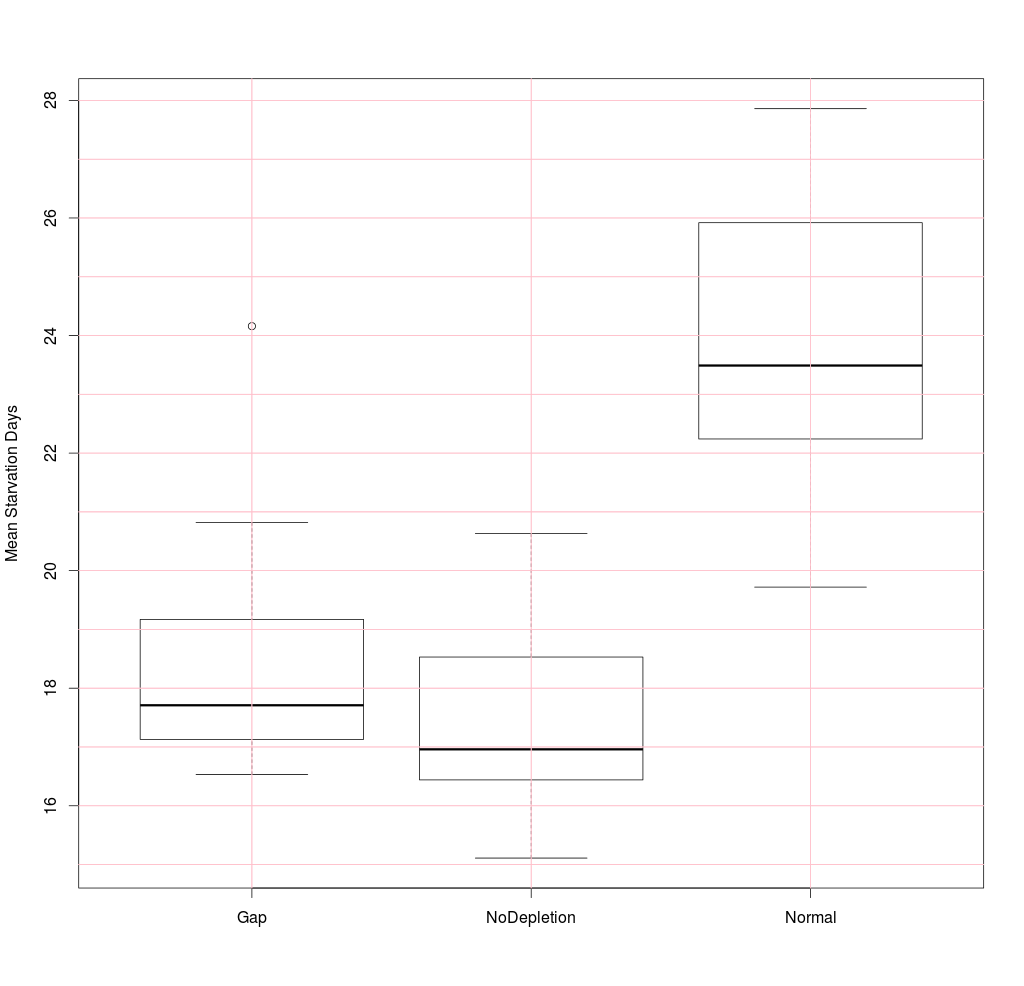
\includegraphics[height=12.2cm]{figures/expm/gapBoxplotsClimate500}
\caption{Mean Starvation days at end of the year box-plots for ``No-Depletion'' experiment 
with 500 rain units at the monsoon season.}
\label{fig:gapBoxplotsClimate500}
\end{figure}


\begin{figure}[!htb]
\centering
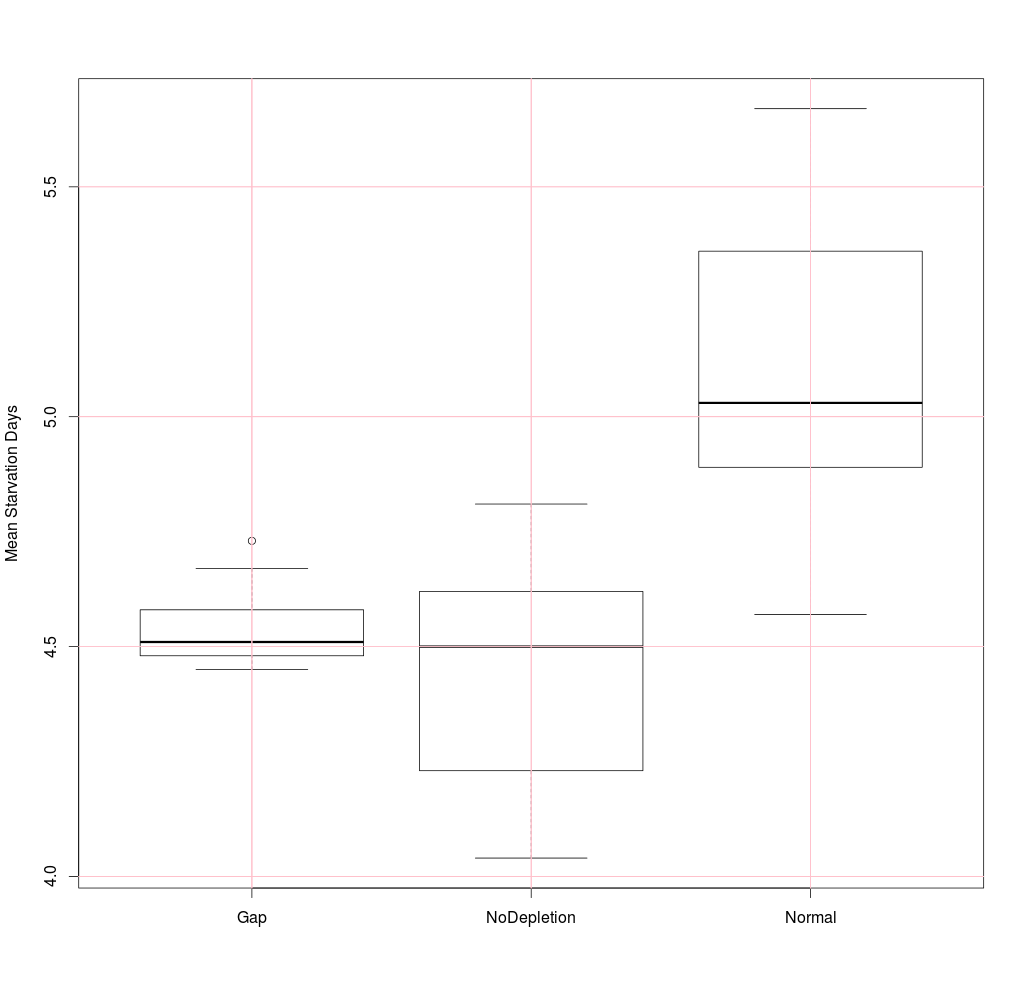
\includegraphics[height=12.2cm]{figures/expm/gapBoxplotsClimate1500}
\caption{Mean Starvation days at end of the year box-plots for ``No-Depletion'' experiment 
with 1500 rain units at the monsoon season.}
\label{fig:gapBoxplotsClimate1500}
\end{figure}


\begin{figure}[!htb]
\centering
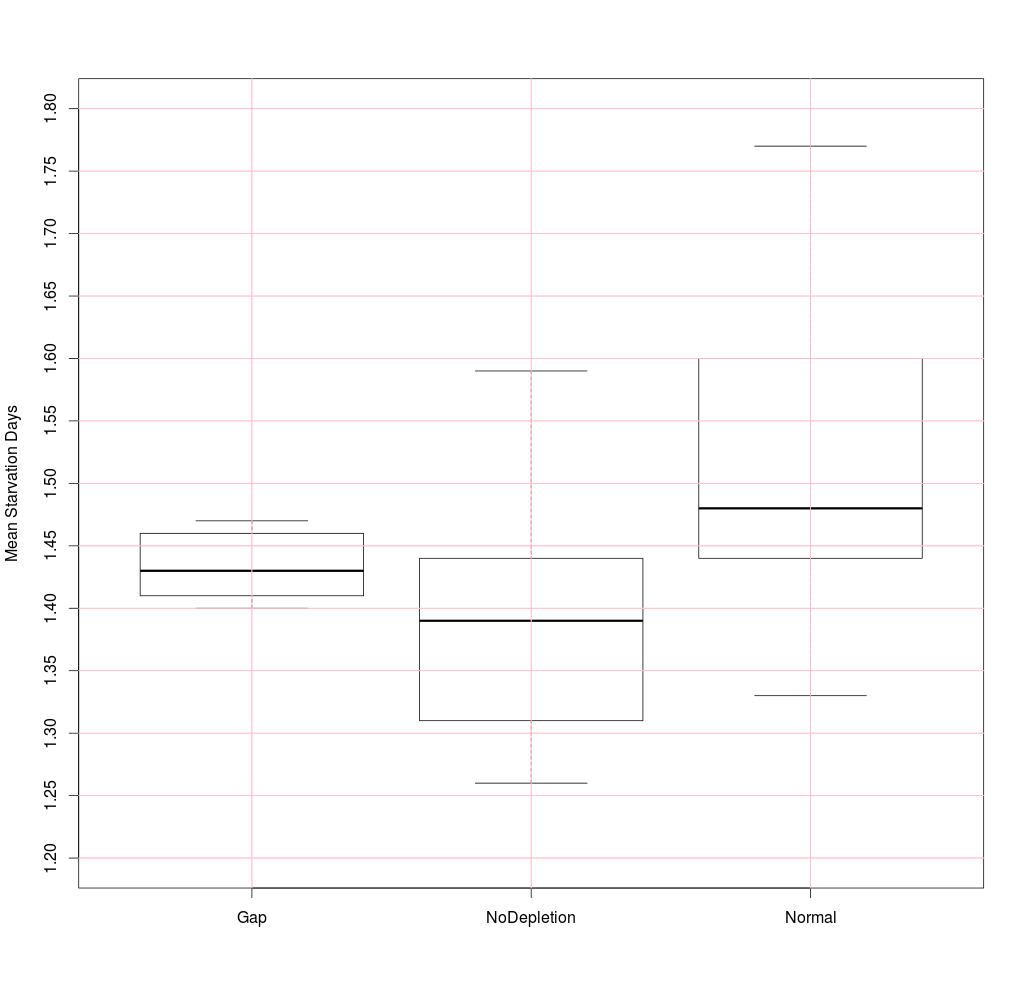
\includegraphics[height=12.2cm]{figures/expm/gapBoxplotsClimate4000}
\caption{Mean Starvation days at end of the year box-plots for ``No-Depletion'' experiment 
with 4000 rain units at the monsoon season.}
\label{fig:gapBoxplotsClimate4000}
\end{figure}


Simulations show indeed that the yearly profile of the starvation rate for the gap agent follows quite 
accurately the profile of the no-depletion agent. Most of the simulations show the pattern of the figure 
when overlapping the Starvation measure for mdp, no-depletion and gap agents corresponding to the same 
simulation seed (Fig.~\ref{fig:gapExplainClimate500}).  

For the different rainfall conditions we kept finding the same result. Box-plots show that the modifications
used in the gap agent approach the performance to the lower bound ( Fig.~\ref{fig:gapBoxplotsClimate500},
Fig.~\ref{fig:gapBoxplotsClimate1500},Fig.~\ref{fig:gapBoxplotsClimate4000} ). 

%%brief conclussion:
In conclusion, there is little space to consider the possibility that more effort applied to biomass 
prediction would reduce the starvation of the agent. The area enclosed between both starvation profiles, the 
normal agent's and the no-depletion agent's is something we must assume due to the design and properties we 
chose to design the model. It is up to future steps to push in the problem of divergence through introducing 
multi-agency and neighbour awareness.


%\pagebreak[4]
\newpage
\section{Comparing the Rule Based Agent and the MDP Agent}

%%Homerange reduit < homerange Gujarat → volem forçat mobilitat ¿per posar al límit els engines?

\subsection{Experiment 1: Mean Starvation Day Comparison}
\label{sec:expEcsi1}
%%quick descrip : 
The first experiment compares the three types, random, rule-based and MDP. The objective is to compare
the performance of different decision mechanisms in movement and foraging activities without interaction
of other agents, without the variability in rainfall, only the end product of survival at the end of a 
short period of time. 
The performance that we measure is directly linked to the critical indicator of survival mechanism, the
measure of mean Starvation days at the end of the year. This measure is affected by the quality of decision
making that the agent makes during the year to get resources to survive.

%%Settings : 
The experiment consists of exploring three amounts of yearly rainfall for a monsoon season at the beginning
of the year. The first scenario tries not to make things easy, 500 units of rain. The second value is mild
and uses a value of 1500 units of rainfall. 
The third scenario replicates the environment that inspired the model, in north Gujarat, with a mean of 4000
units of rainfall, and standard deviation of 2000 units. The standard deviation is not used in this two year
simulation but it is applied in the ten years simulation of experiment two. As it is mentioned, the simulation
lasts two years. 
We hope to giving the agent time to explore and discern a patch during the first year with a minimum quality
to see how they develop during the second year of the three engines that decisions are being compared. All 
runs start with the agent located in the upper left of the map, with two adults and four children. MDP agents
are configured with the following combinations of parameters, horizon 10 plus width 1000, horizon 3 plus 
width 500, horizon 6 plus width 1000 and horizon 6 plus width 500.
We simulate runs with one single agent because do not want the noise introduced by other neighbours in the
analysis of the agent getting on in the foraging and migration activities.

The data from the experiment is distributed producing a figure for each different rainfall.
Each climatic condition contains a set of juxtaposed box-plots. 
Each box-plot is the statistical summary of starvation rate for one configuration of agent engine. The 
adjacent placement allows us to compare the deviation of the distributions and their averages.

\begin{figure}[!htb]
\centering
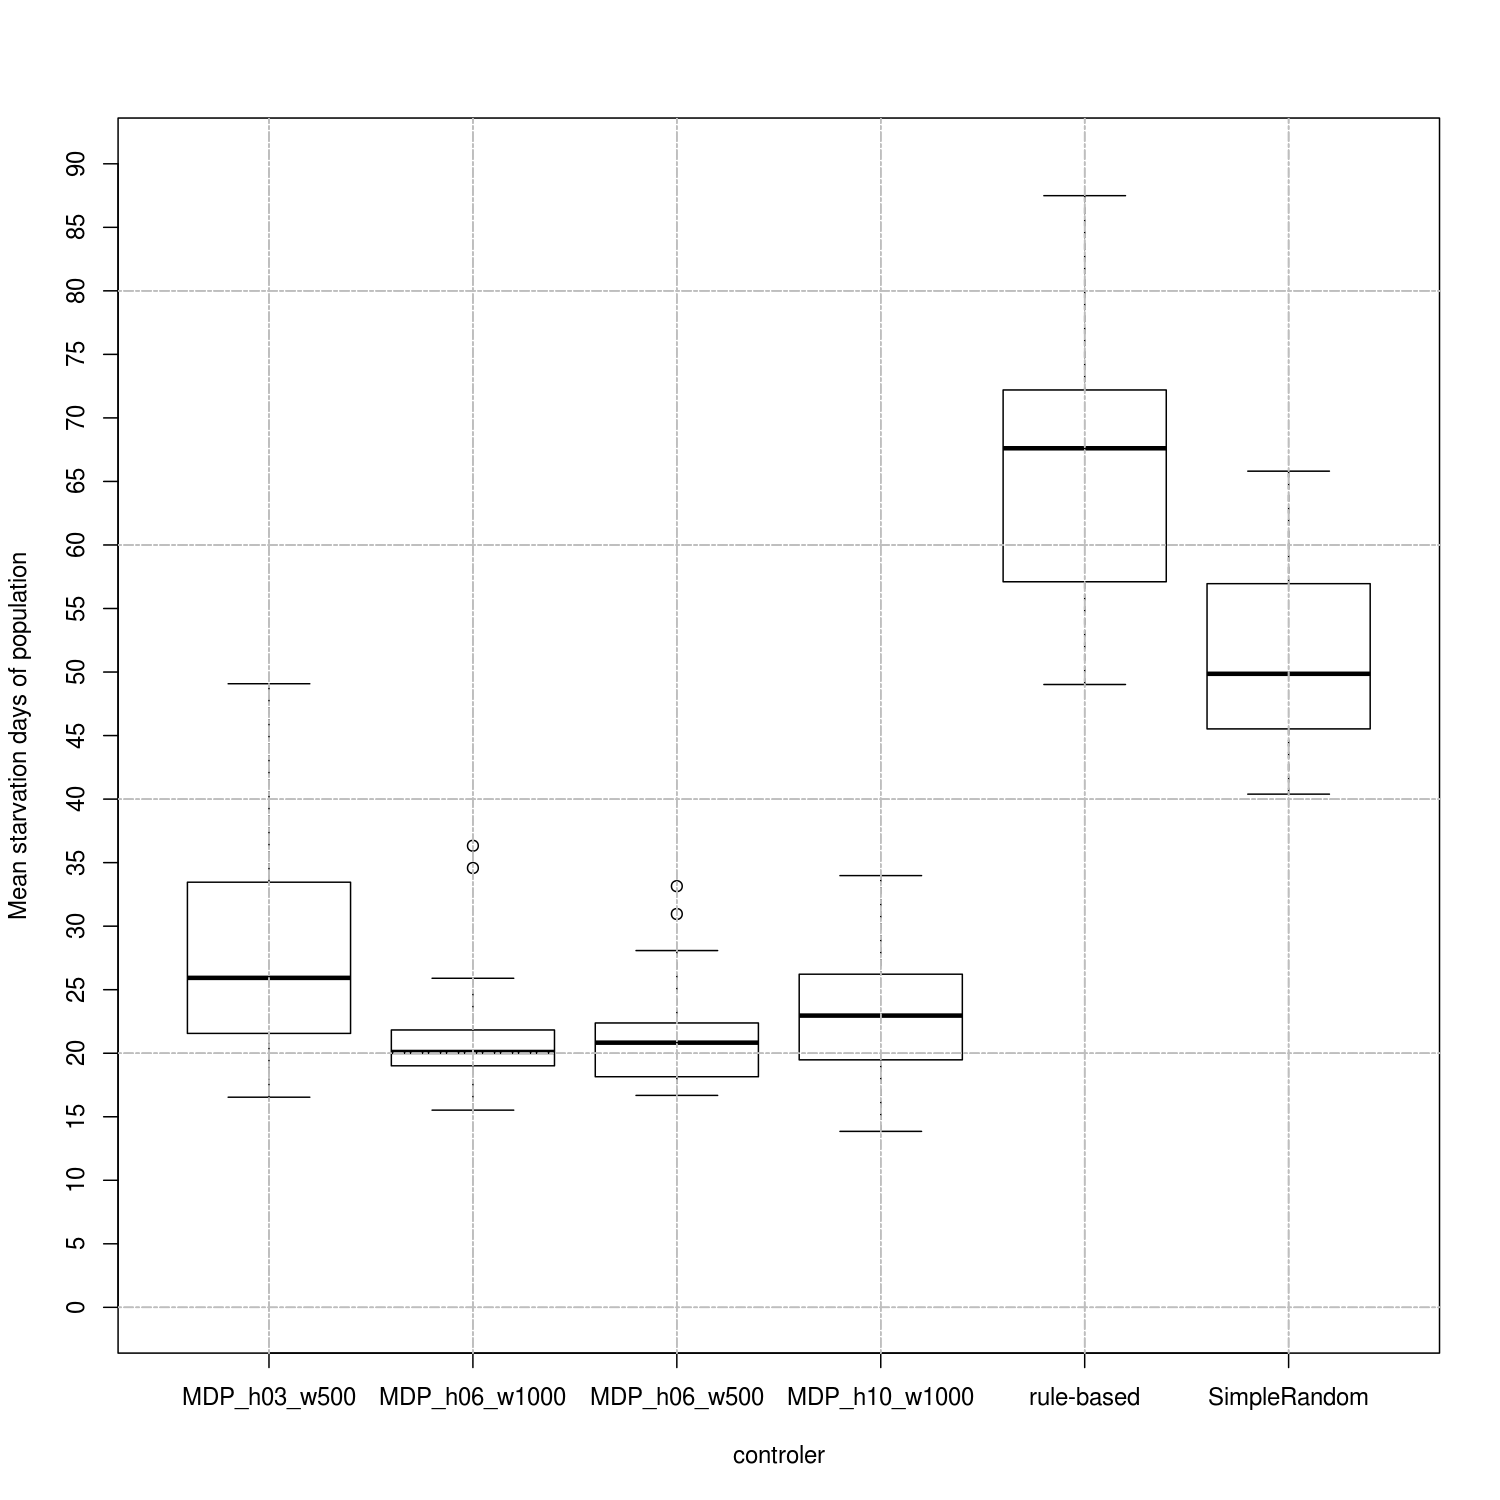
\includegraphics[height=12.2cm]{figures/expm/ecsi1_clim500}
\caption{Mean Starvation days for a rainfall of 500 units}
\label{fig:ecsi1_clim500}
\end{figure}

\begin{figure}[!htb]
\centering
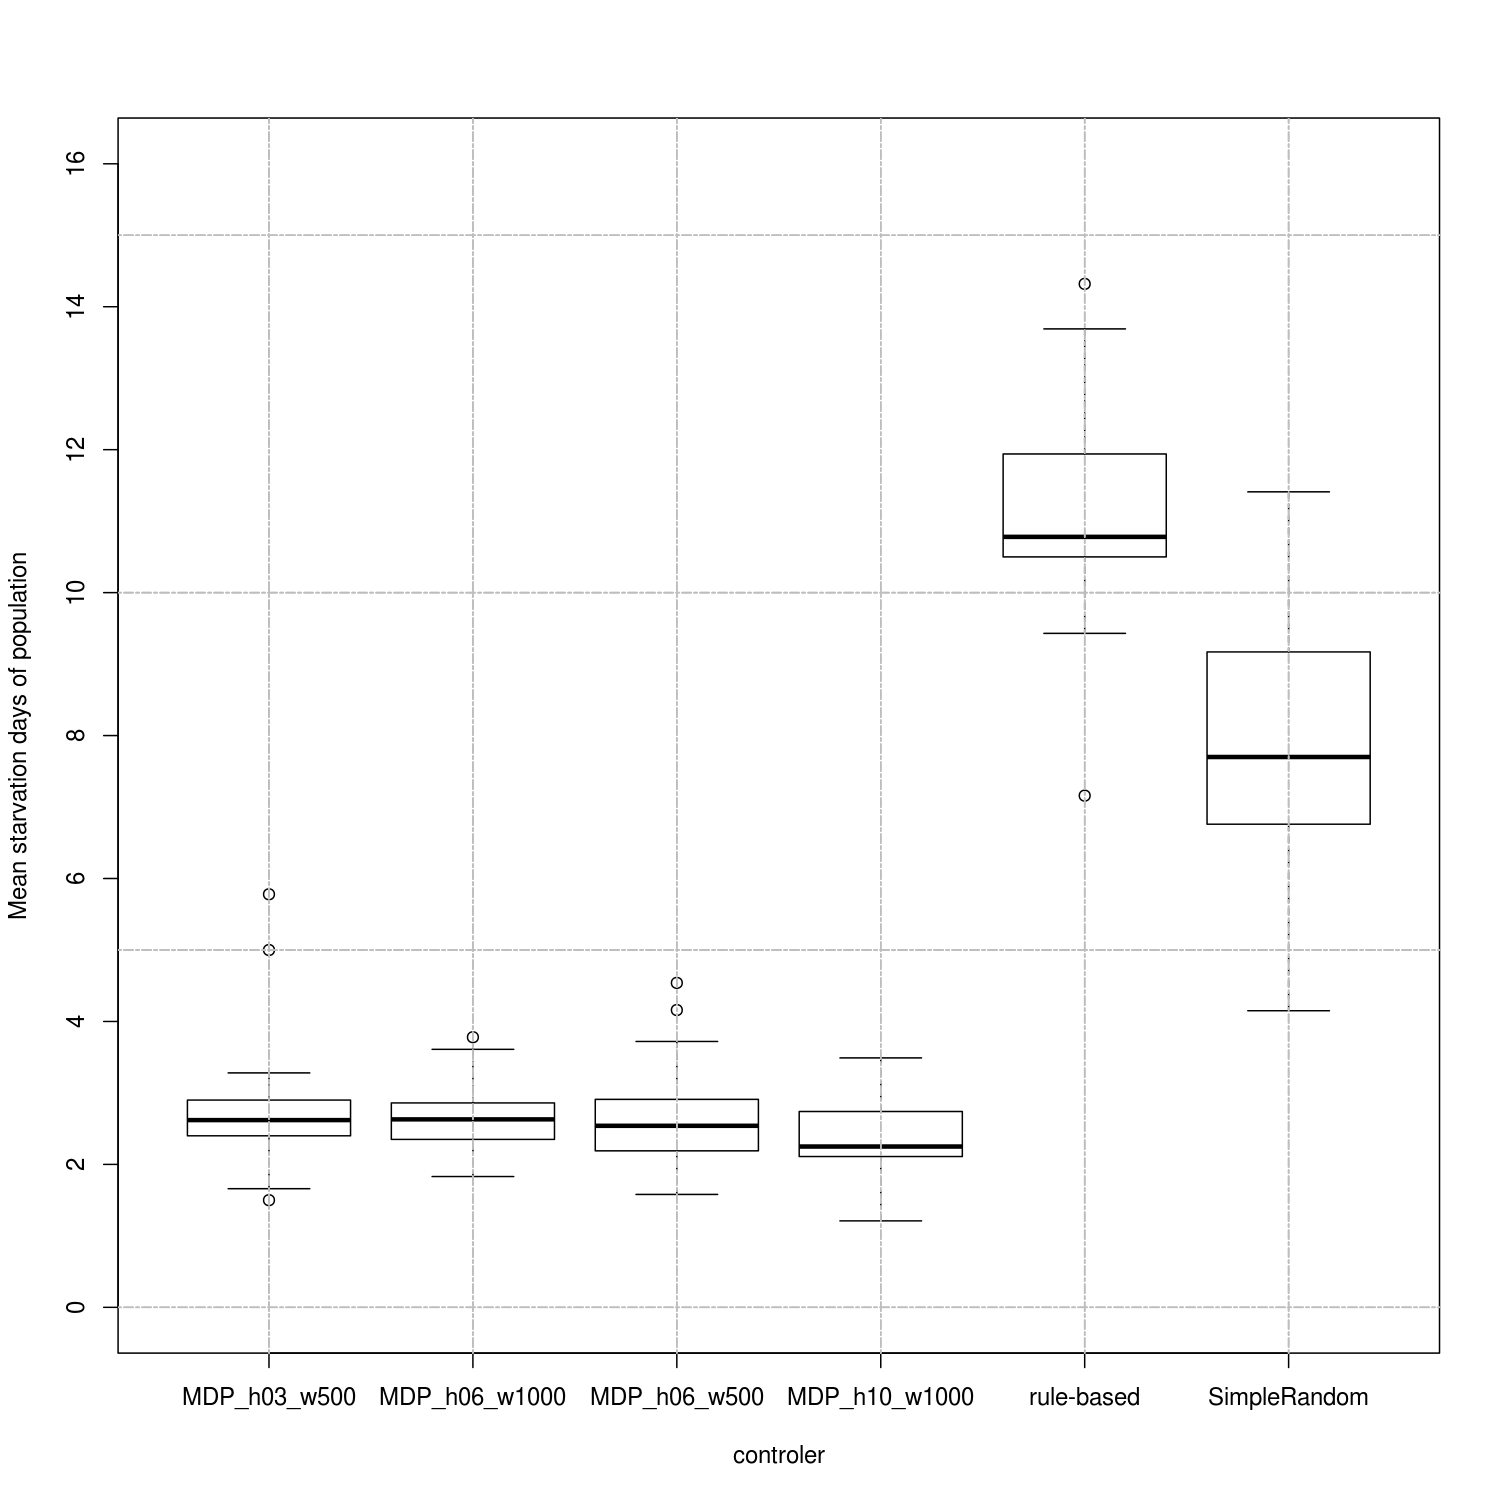
\includegraphics[height=12.2cm]{figures/expm/ecsi1_clim1500}
\caption{Mean Starvation days for a rainfall of 1500 units}
\label{fig:ecsi1_clim1500}
\end{figure}

\begin{figure}[!htb]
\centering
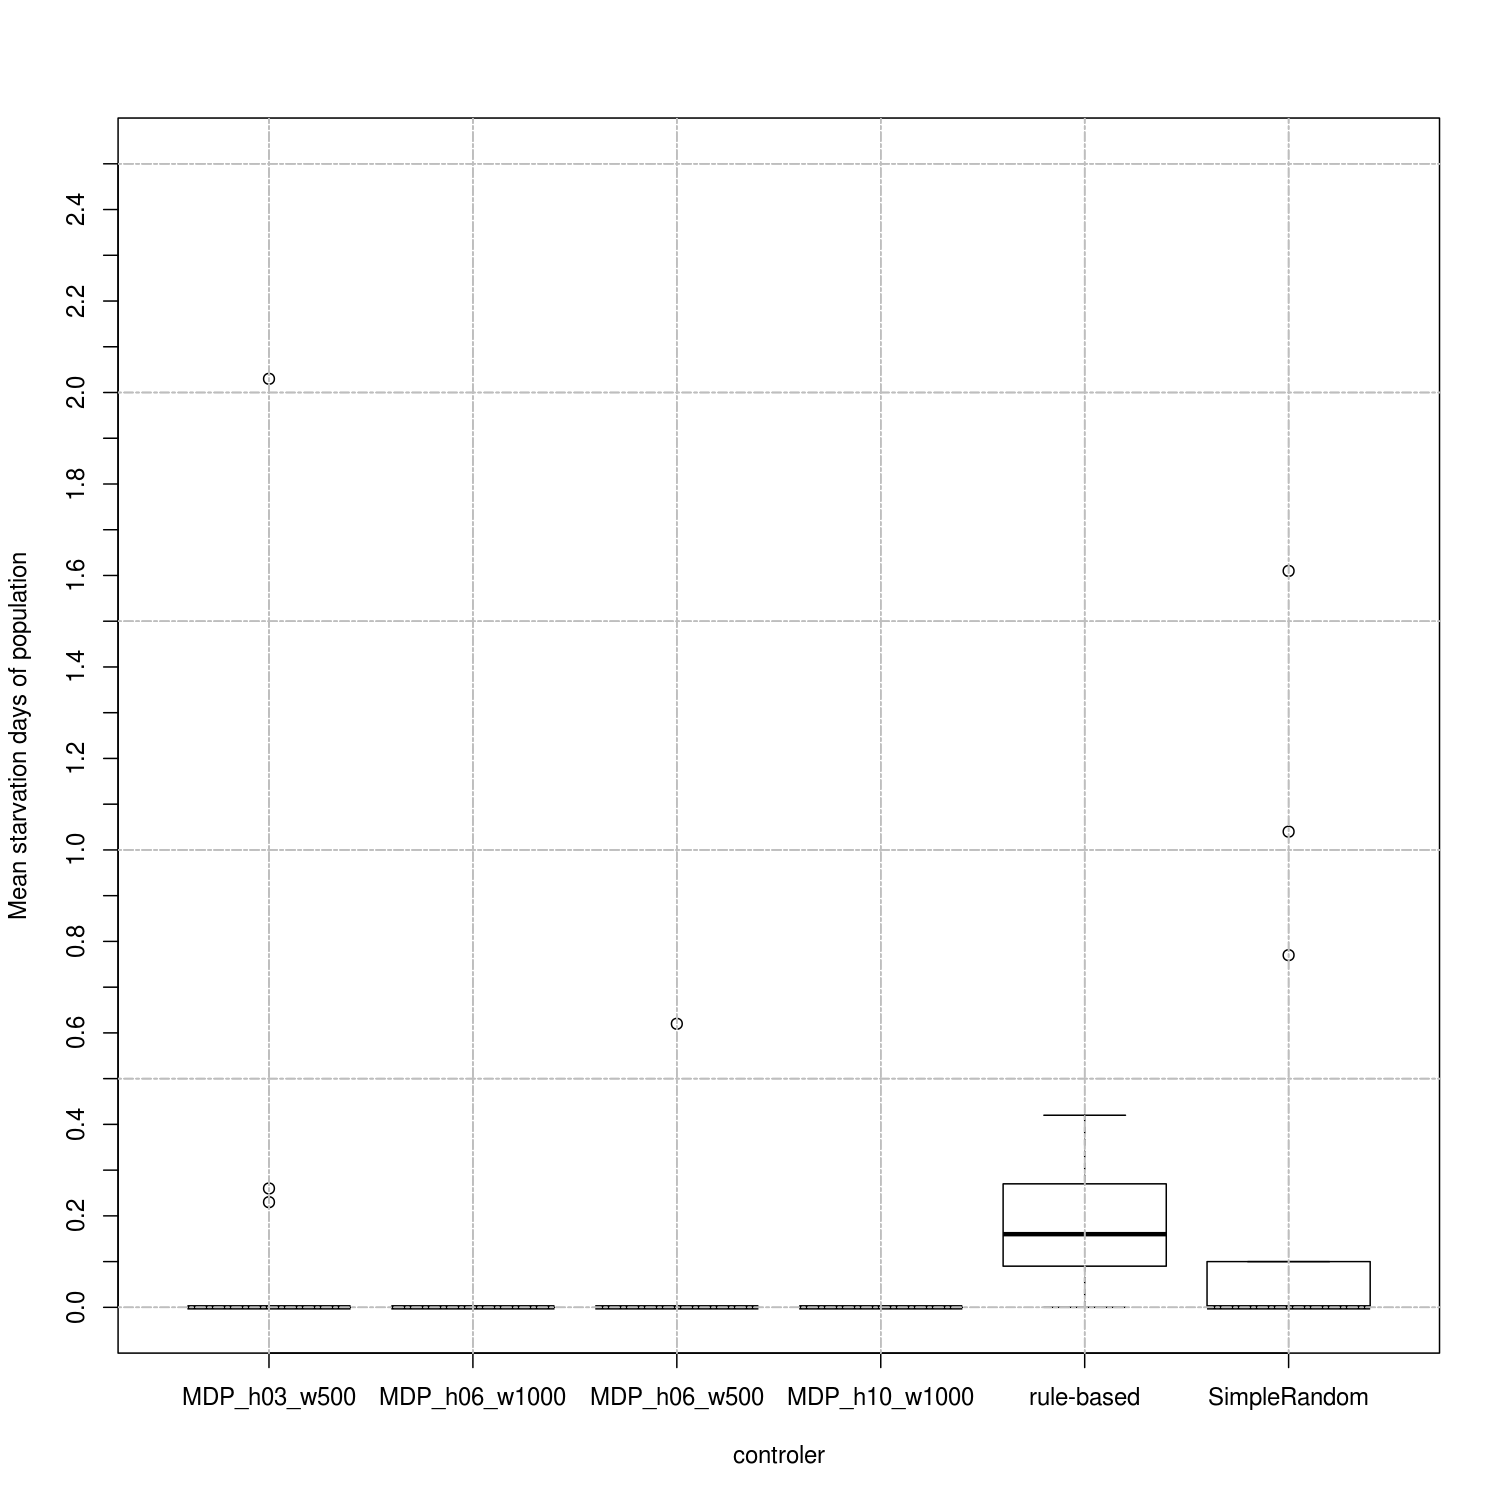
\includegraphics[height=12.2cm]{figures/expm/ecsi1_clim4000}
\caption{Mean Starvation days for a rainfall of 4000 units}
\label{fig:ecsi1_clim4000}
\end{figure}


%%describe plots : 
We can clearly see that the rule based agent obtains the worse score in starvation rate (Fig. ~\ref{fig:ecsi1_clim500},Fig. ~\ref{fig:ecsi1_clim1500},Fig. ~\ref{fig:ecsi1_clim4000}). All the mdp configurations get lower values respect the rule based and random agent.

%%brief conclussion/observations: 
MDPs exhibit a better performance than other agents. In the long term they will die from two to four times less than the classical approach of reactive rules.
Also, we have been surprised by the better performance of the Random agent versus the rule based. We can offer an explanation to this based on movement rate and penalty due to movement. Agents produce chains of movement actions and foraging actions. 
One foraging action occupies the working time of a day. One movement action produces movement and some resource retrieval that could be understood as foraging along the trip path. We have represented it as a half reward from a secondary foraging action bonded to the movement action that take place in the same day.

It is critical to know the correct time-lapse when to move the settlement: The day you move you will only retrieve half of the resources you could take in a normal day of only foraging. As days pass you deplete your home range till the time step that you cannot make a living from the resources around home. 
For the rule based agent that is the condition to move. If you move when resources are under your survival threshold the “half reward” associated to a movement day will be much more below your survival threshold; and it is a severe penalty. 
If you tune the decision rule to avoid an extreme depletion of the surrounding environment you will have an agent that moves too much which leads to half- reward penalty accumulation.


\begin{figure}[!htb]
\centering
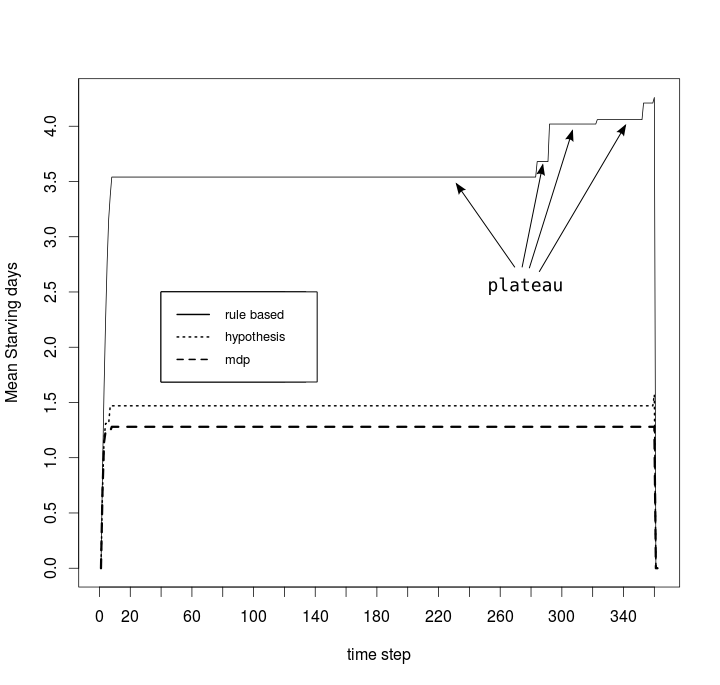
\includegraphics[height=12.2cm]{figures/expm/BW_markovMoveHypothesis_TAGGED}
\caption{Starvation rate profile along a year for three types of agent. The higher the value, the worse.}
\label{fig:markov_move}
\end{figure}


The figure (Fig.~\ref{fig:markov_move}) shows a typical profile of mean starvation along a year for three kind 
of agents, a rule based one, an mdp agent, an the one called hypothesis. Starvation increases in the firsts 
days of the year from zero to some value that will be hold till the critical part of the year. The resource 
dynamics depends on the first season of monsoon. At the beginning it rains but there are no resources. It 
explains why starvations increases in the first days. And the last season of the year is a dry one where 
resource are scarce or practically zero. Taking into account only the rule agent and the mdp we can see there 
is no way to get a zero starvation score. There are no resources whether you move one place or another, there 
is no smart path selection that will give more resources when there is practically nothing. Any path of 
movement leads to low resource patches. That is why for both agents there is an increase on their starvation 
ratio in the first days of the year. But, why is it higher for the rule based? Because the rule based agent 
moves when it finds resources are under the threshold condition on the movement rule. The agent will move and 
will receive the penalty of the half-forage. By the other hand, the mdp agent can explore plans and detect the
ones that will make arise the penalty associated to movement actions it is not advisable to move. The mdp 
agent waits. For the central part of the year there are enough resources and both type of agents can manage 
well. But again, when there are low resources around the rule based agent will not behave optimally. In a 
first approach one could think that you cannot scape from starvation, there are low resources like at the 
beginning of the year. Au contraire,the presence of plateaus tagged in the profile of the starvation indicate 
that for some steps the agent does not see its starvation rate increased, so there are enough resources to 
survive for some days. The plateaus are correlated with the movement actions. And each time we have seen a 
change from one plateau to another one there have been movement. These increments come from the penalty 
associated to half rewards the days you move. The rule based agent waits till it is too late and there so low 
resources that moving implies to receive a half-reward under the survival threshold of resources. 
The mdp agent can manage to choose the time-step to move minimizing the penalty and moving before it is too 
late while there are enough resources and a half-forage will not be as harmful as if you have waited too much. 
We checked this hypothesis extending the rule based agent with two new rules. The rules are inspired in the 
mistakes shown by the rule based agent. The first extra rule says “At the beginning of the year do not move 
till time-step 7”. The second rule says “If last move action was launched more then 5 steps ago, move now”. 
The extended rule agent corresponds to the dotted profile in the figure(Fig. ~\ref{fig:markov_move}) with the label “hypothesis”. 
It is not our aim to enhance the rule based agent adding more and more rules, because many times any set of 
rules will have a fail point that can be triggered by the changing conditions of the environment. But the 
important thing is that through this comparison, apart from checking one agent type versus the other, we 
obtained a deeper insight of the system, of the mechanics and conditions for correct resource depletion. 
And this is a by-product of putting side by side different decision making engines. 

Besides, we also observed that configurations with horizon 6 in mdp agents performed like horizon 10 
configurations. Our hypothesis is that after doing some statistics the size of time lapse between consecutive
move actions is approximately five or six steps in mean, or even less for the last days of the year, when resources are more scarce. It seems that the optimal time to exploit resources in a patch is no more than four
or five days, then, if you exceed this bound you must leave launching a move action (as previously mentioned). 
The decision process must foresee the best time step to move paying the minimum penalty. And if the horizon 
covers such time lapse between move actions  it will cover the feasible days inside the set to choose the day
with optimal balance of minimum penalty and maximal normal forage reward.  

To assess this explanation we produced some density plots  (Fig.~\ref{fig:segmLength_clim4000_begin320} for a 
rainfall of 4000 units), (Fig.~\ref{fig:segmLength_clim1500_begin320} for a rainfall of 1500 units),
(Fig.~\ref{fig:segmLength_clim500_begin320} for a rainfall of 500 units). For each run from the experiment, 
the amount of time steps(time lapse length) between move actions is registered . But we only consider time 
steps from the critical part of the year, the last forty steps.
Each run will have a mean of lengths associated. For each configuration of the mdp agent we will have a set 
of means of lengths. This set is a sample of the distribution that will characterize a configuration. 
Each run is a two year simulation from the experiment 1 we are describing in this section. We took each set 
of means and produced a density plot for the distribution of mean lengths for each different horizon, three, 
six and ten.The more two density plots match the more we could guess that the distribution of sequences of move actions match and that the two compared configurations produce plans that are not very different one from another.



\begin{figure}[!htb]
\centering
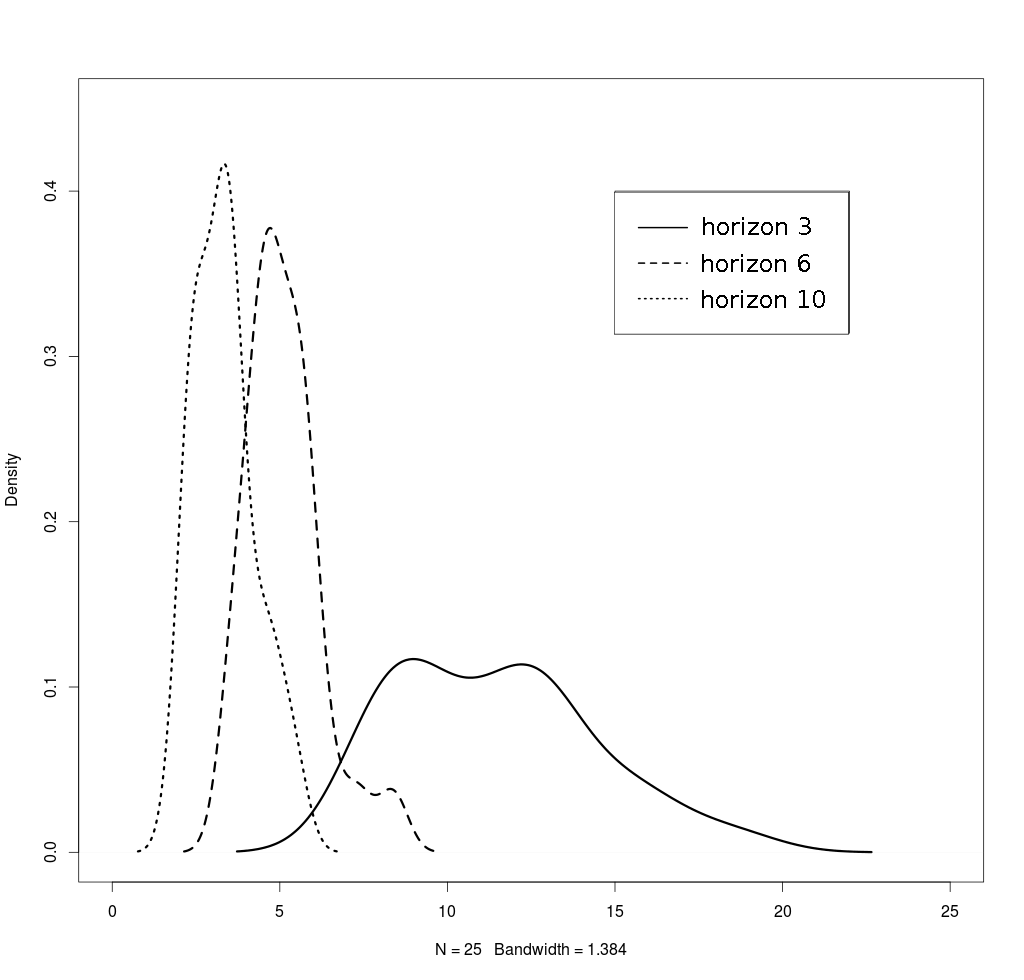
\includegraphics[height=12.2cm]{figures/expm/segmLength_clim4000_begin320}
\caption{Density distribution for time lapse length between move actions for a rainfall of 4000 units.}
\label{fig:segmLength_clim4000_begin320}
\end{figure}

\begin{figure}[!htb]
\centering
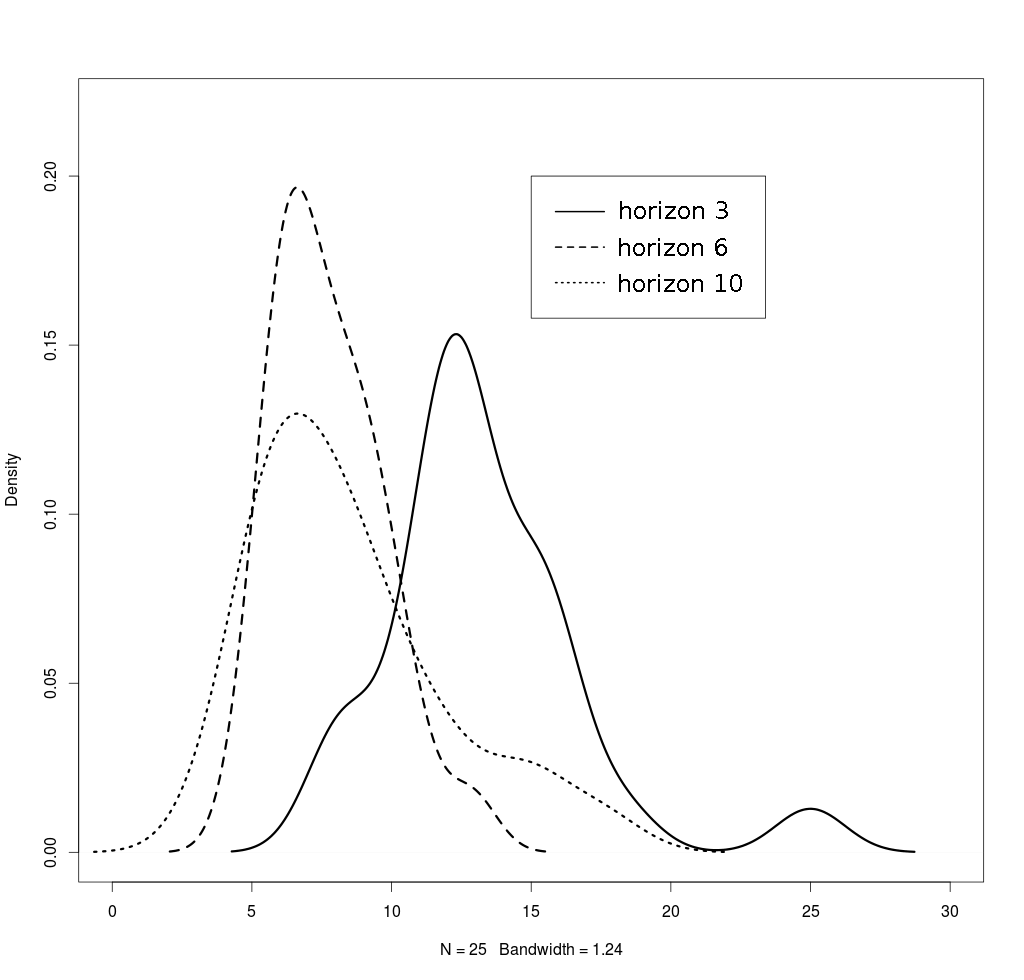
\includegraphics[height=12.2cm]{figures/expm/segmLength_clim1500_begin320}
\caption{Density distribution for time lapse length between move actions for a rainfall of 1500 units.}
\label{fig:segmLength_clim1500_begin320}
\end{figure}

\begin{figure}[!htb]
\centering
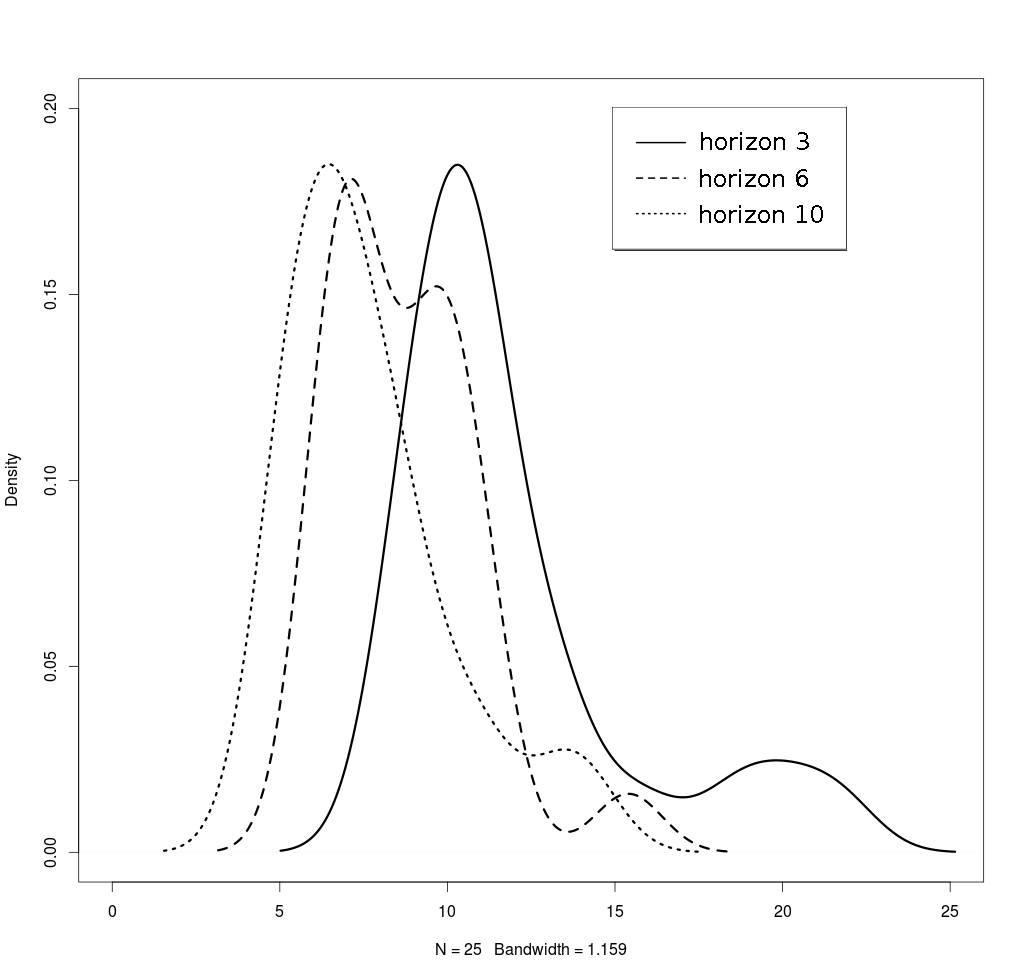
\includegraphics[height=12.2cm]{figures/expm/segmLength_clim500_begin320}
\caption{Density distribution for time lapse length between move actions for a rainfall of 500 units.}
\label{fig:segmLength_clim500_begin320}
\end{figure}


The plots strengthen the evidence that configurations horizon 6 and horizon 10 besides having similar starvation and hence, survival performance, they have plausible matching distributions of lengths.


\subsection{Experiment 2: Ten year simulation of Rule Based Agent vs MDP Agent}
\label{sec:expEcsi2}
%%quick descrip : 
The second experiment extends the simulation from two year runs to ten year runs. 
A longer run will make explicit the response to accumulated changes through the years, mainly, the dynamics of individuals that conform the agent, as new children are born or some die due to starvation or the demographic mortality basic rules. 
%%Settings : 
We replicate the settings and configurations used in the first experiment, except that the random agent is not taken into account; we focus on comparing the drift of the classical rule agent with the mdp agent.

%%describe plots :

The ten year trace (Fig.~\ref{fig:popClim500_BW} for a rainfall of 500 units, Fig.~\ref{fig:popClim1500_BW} for a rainfall of 1500 units, Fig.~\ref{fig:popClim4000_BW} for a rainfall of 4000 units), contains a set of cells with a number indicating the year on top of them.
For each year there will be a set of box-plots of the mean of starvation rates. The Y axis is the measure for starvation and the X axis contains the spread of configurations evaluated. The box-plots follow the order in the legend.
The top most item of the legend, configuration ''h3\_w100'' ( horizon 3, width 100 ) corresponds to the most left box-plot in a year cell. As we go down in the legend we find the configurations that appear in a sorted manner from left to right. 

\begin{figure}[!htb]
\centering
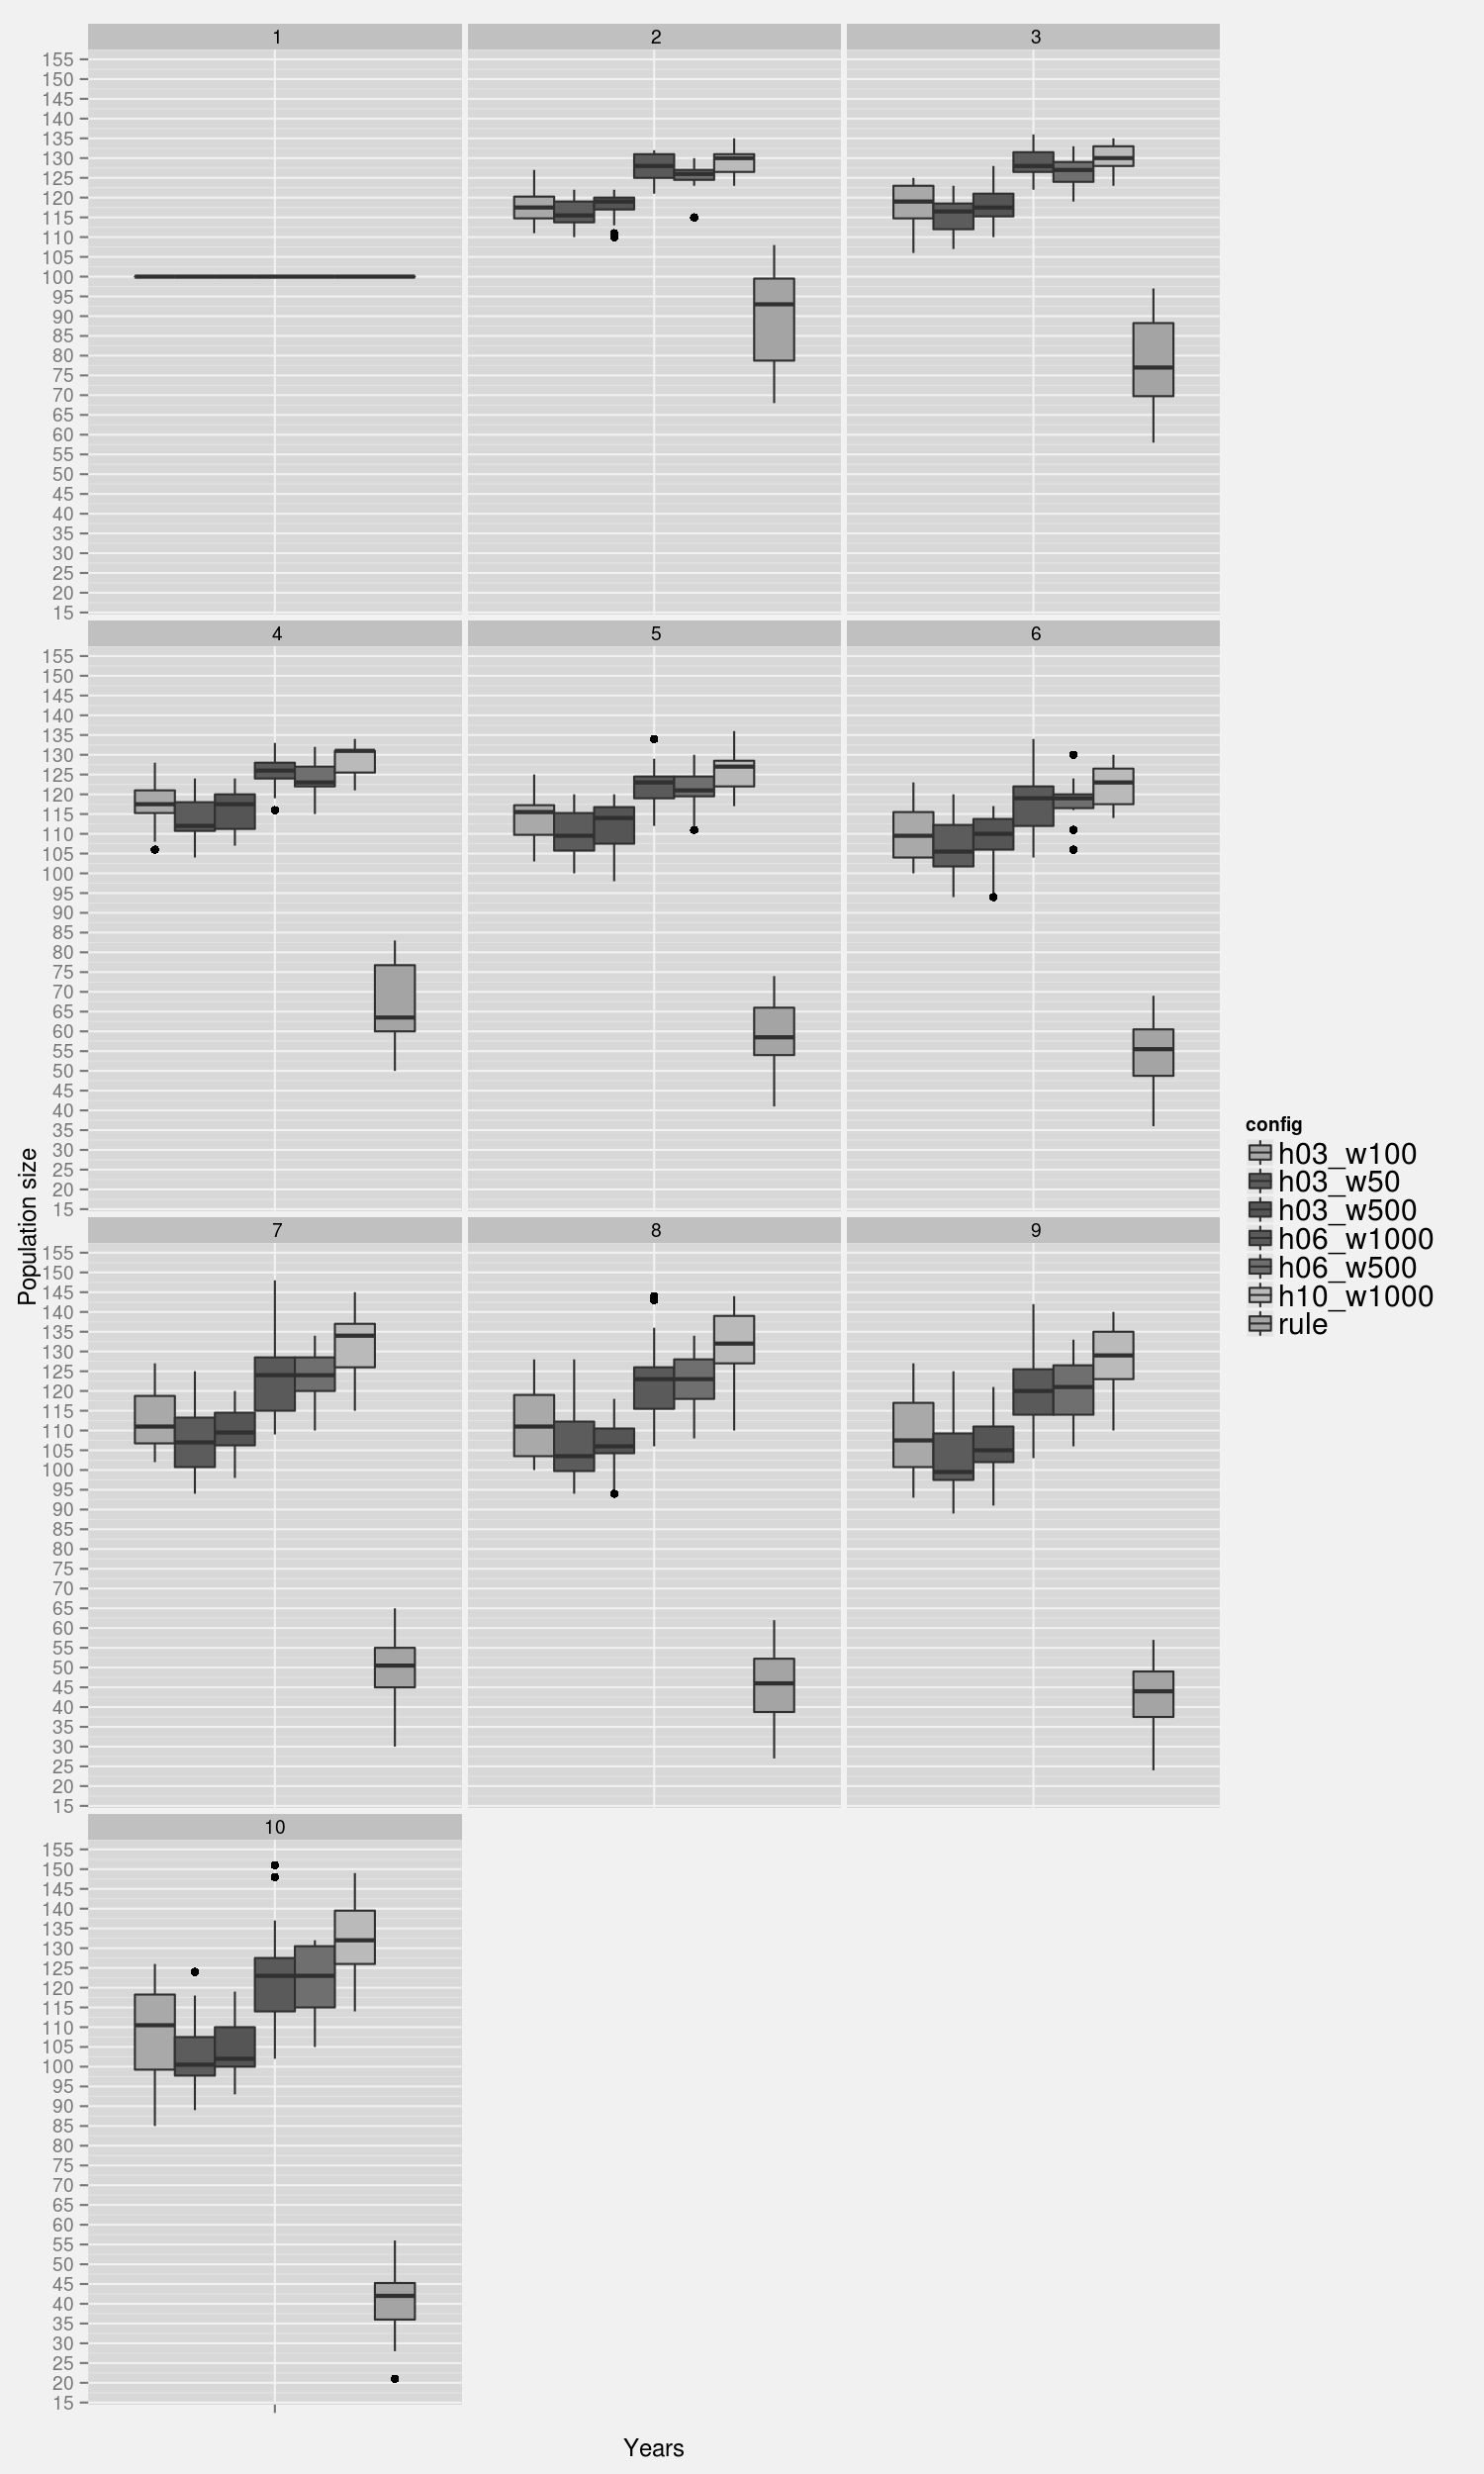
\includegraphics[height=20.2cm]{figures/expm/popClim500_BW}
\caption{Trace of starvation rate along a ten year simulation with one hundred agents. The resources are produced by a rainfall of 500 units.}
\label{fig:popClim500_BW}
\end{figure}

\begin{figure}[!htb]
\centering
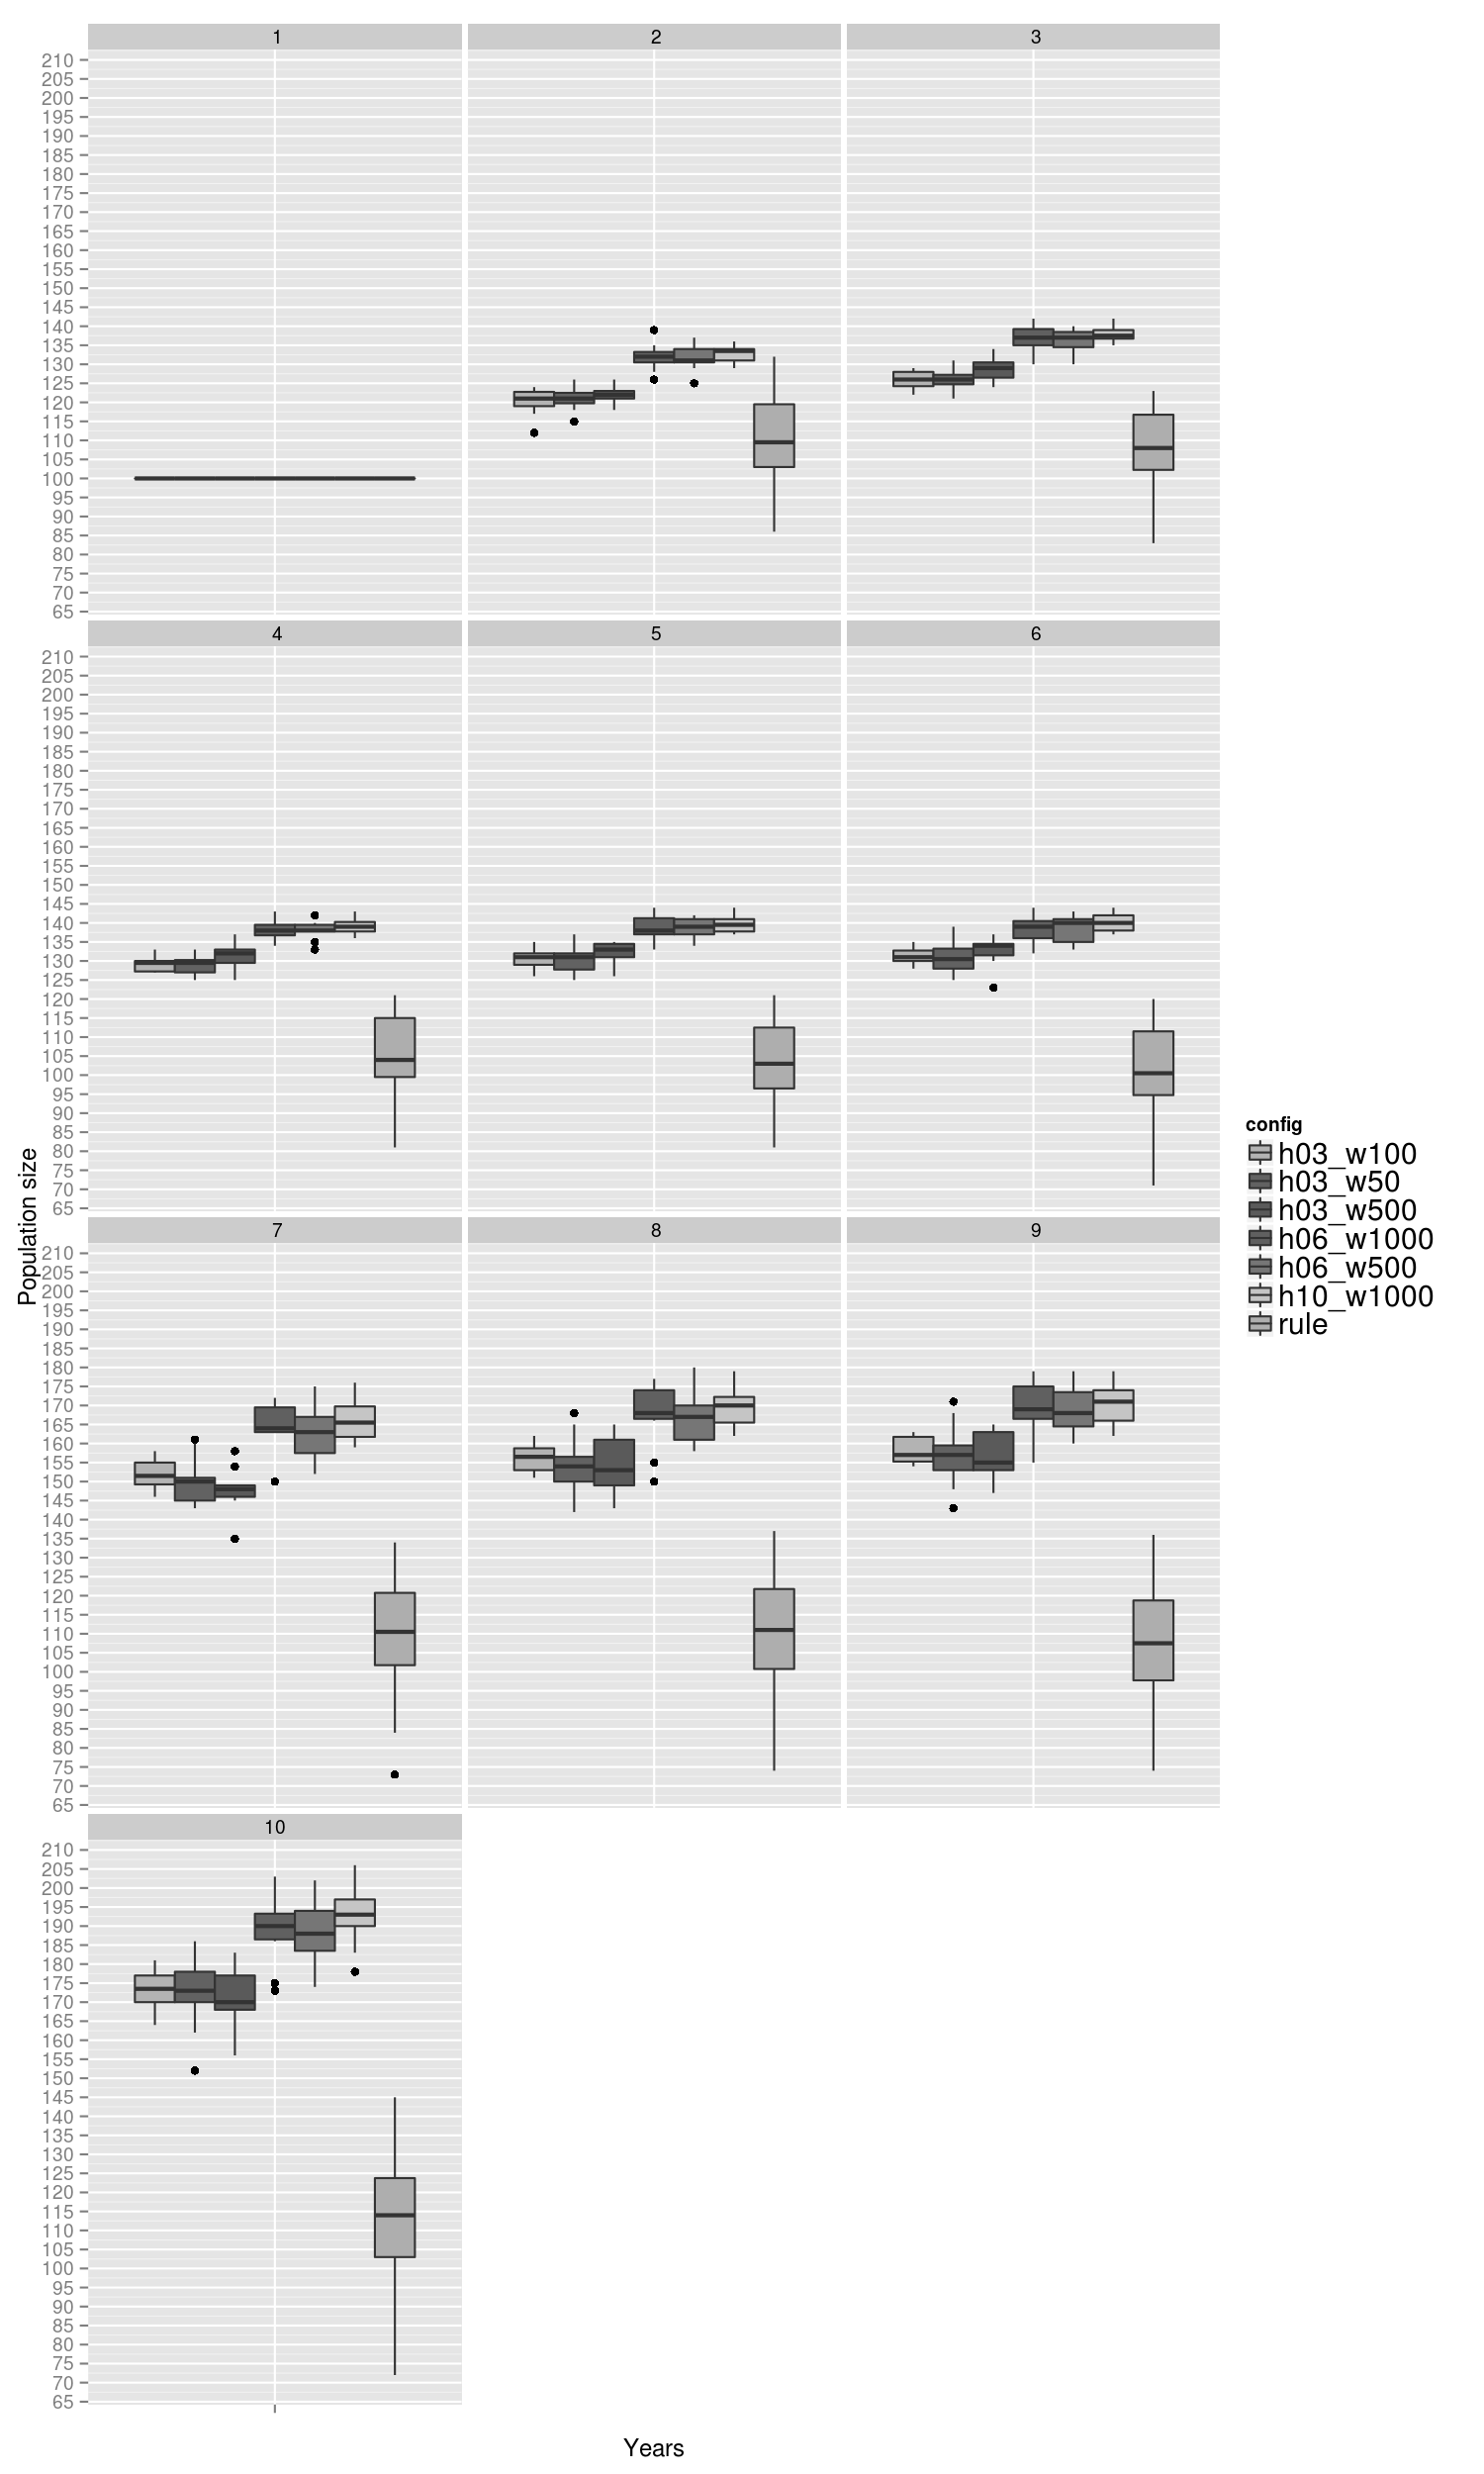
\includegraphics[height=20.2cm]{figures/expm/popClim1500_BW}
\caption{Trace of starvation rate along a ten year simulation with one hundred agents. The resources are produced by a rainfall of 1500 units.}
\label{fig:popClim1500_BW}
\end{figure}

\begin{figure}[!htb]
\centering
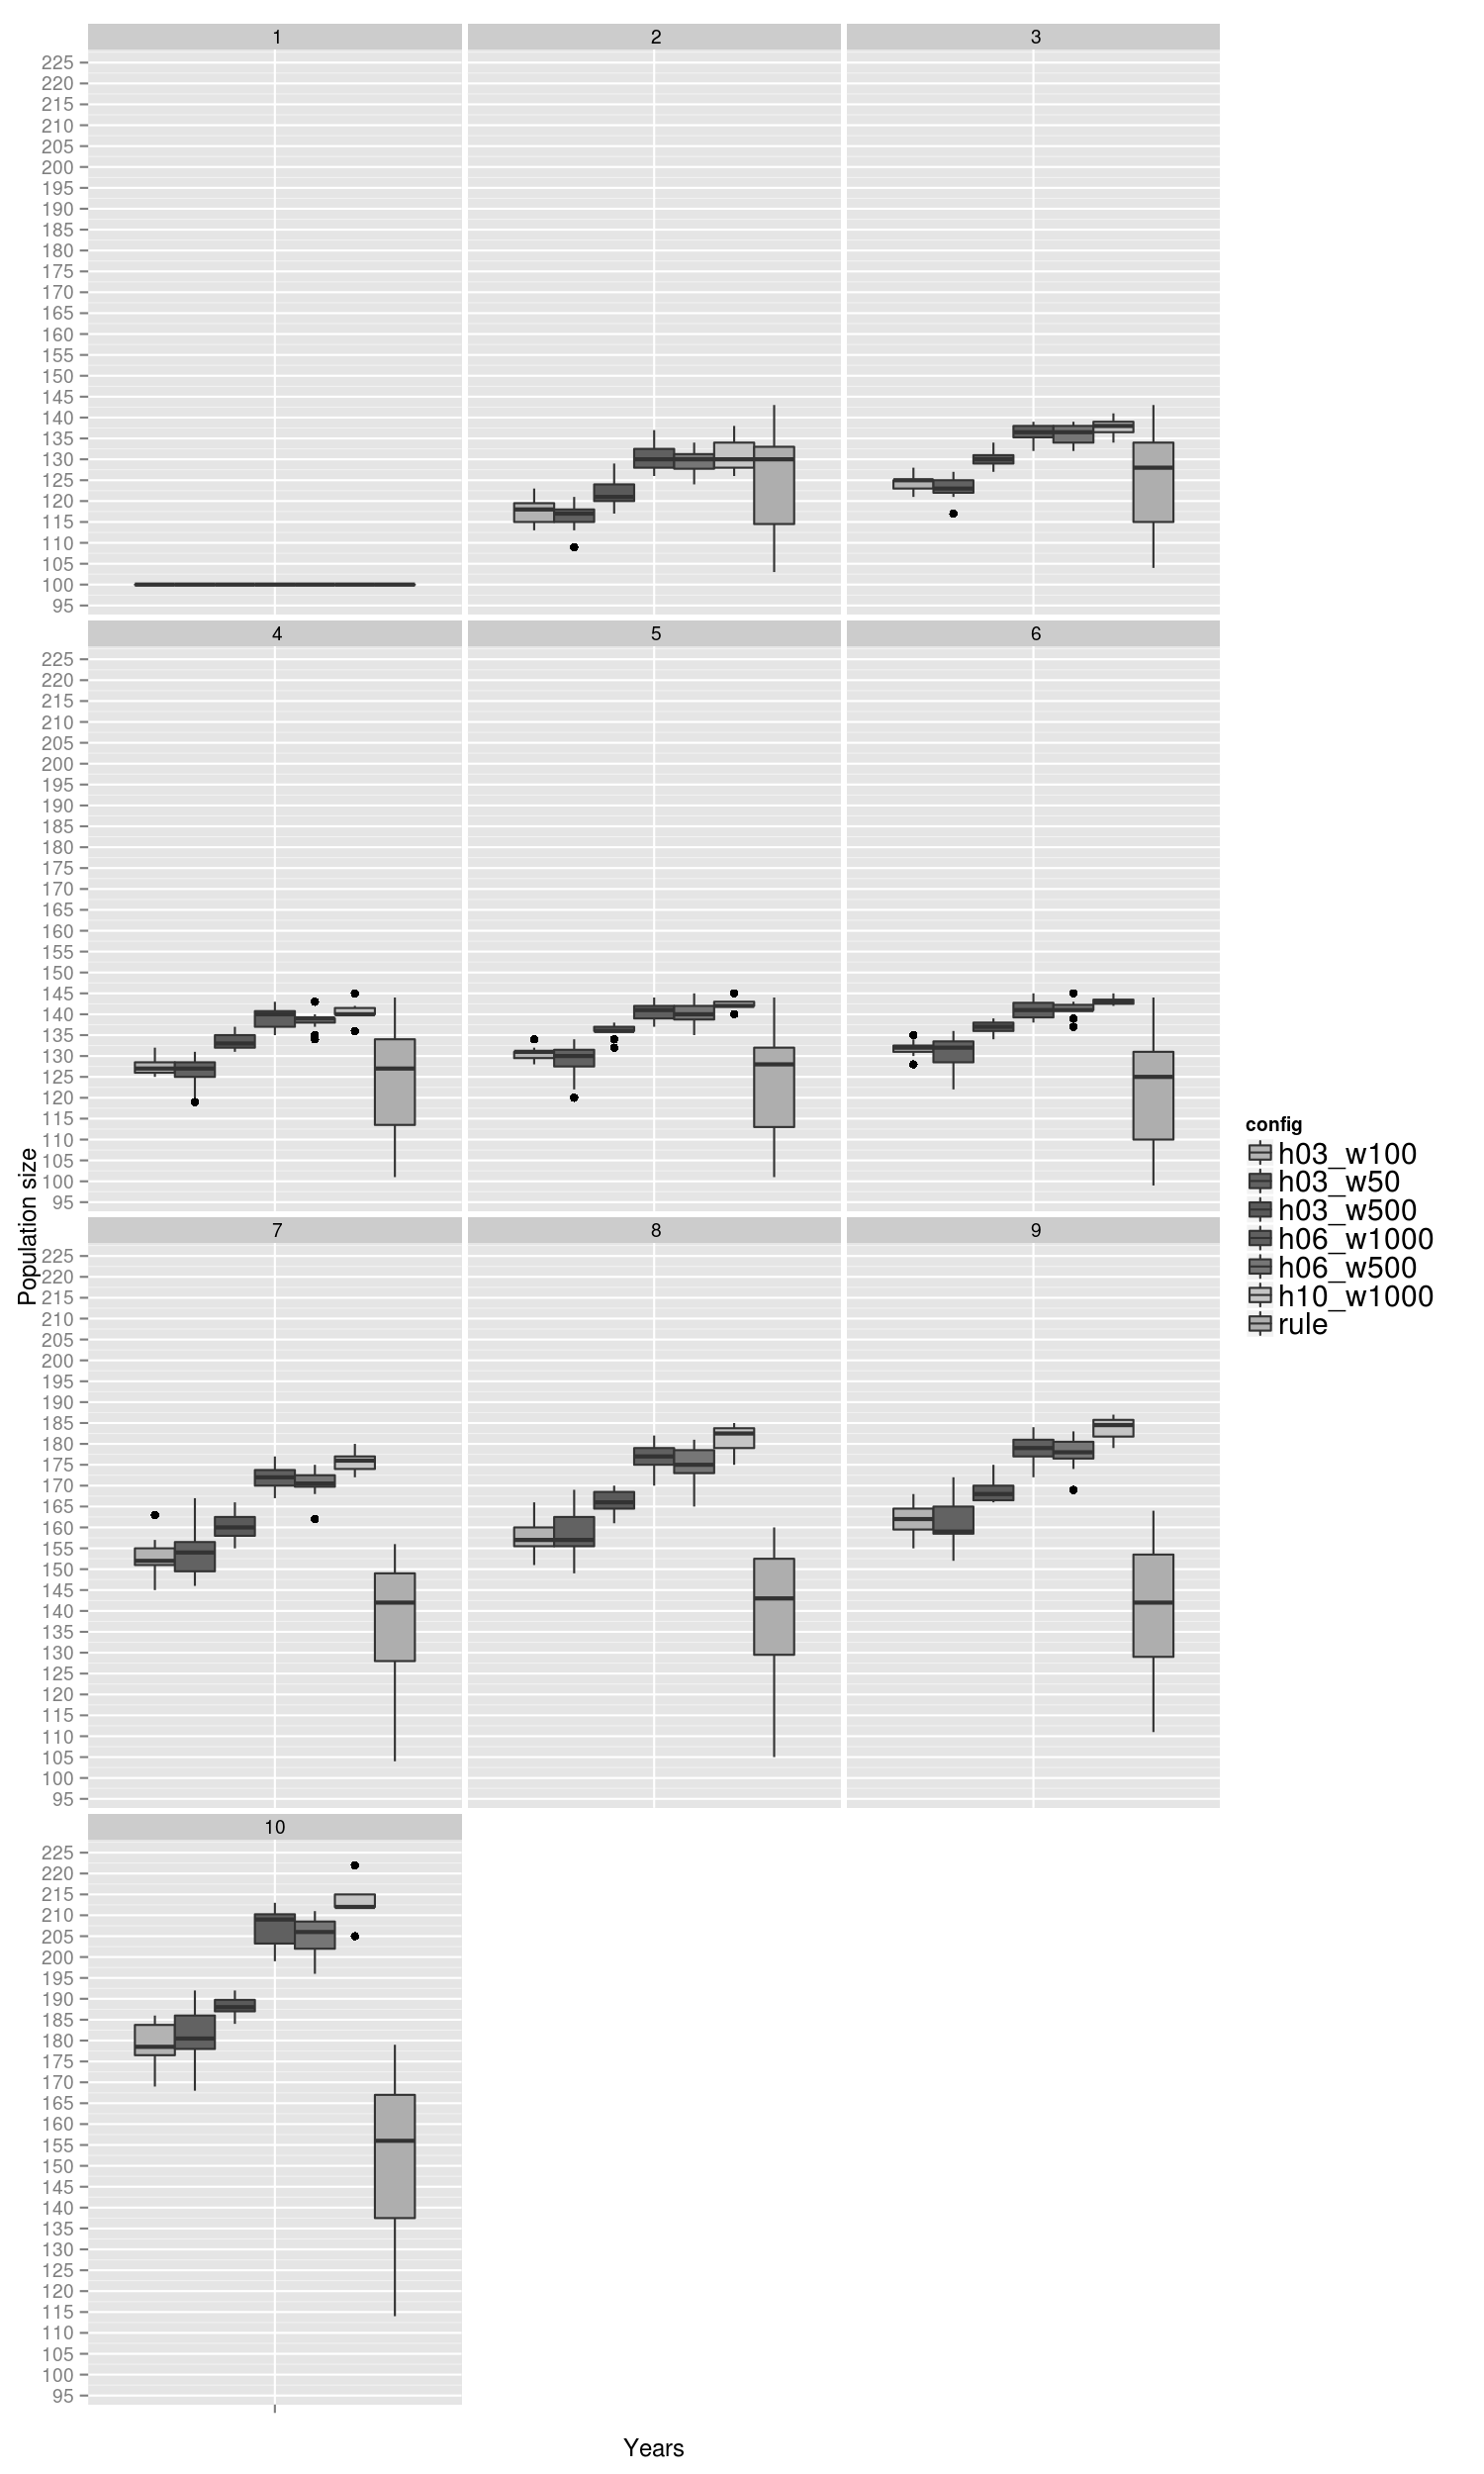
\includegraphics[height=20.2cm]{figures/expm/popClim4000_BW}
\caption{Trace of starvation rate along a ten year simulation with one hundred agents. The resources are produced by a rainfall of 4000 units.}
\label{fig:popClim4000_BW}
\end{figure}


Box-plots for configurations from mdp agents appear clustered in two sets. The horizon 3 set and the  horizon 6 and 10 set. As we expected the rule based agent falls apart and exhibits a very different trend from the mdp agents. For the scenario with rainfall set to 500 the mdp agents thrive towards to an increase of population that maybe will settle in the carrying capacity. 
But, the rule agent follows a decrease that by the last year gives us a first case that does not see its agents alive, the black dot under the rule based's box-plot at level zero. We could conclude that with enough time the rule based group will collapse although the decrease rate is asymptotic to forty. For the plot with rainfall 1500, things get easier and probably the rule based agent group would not collapse and remain stable around a population of one hundred fifteen.  
The third scenario is very friendly for agents, there are enough resources for groups of one hundred agents and all the types we are comparing evolve to greater sizes in their populations. The rule agents can not enjoy a same growing rate as the mdp ones.
Let's see that as we increase rainfall the deviation in the box-plots of mdp agents decreases. There are more resources and it masks the depletion of the other agent for some agent that most calculate its plan. This reduces uncertainty and stochasticity in the rewards and starvation rates.

%%brief conclussion:
The differences between the classical approach and the AI approach arise more explicitly in experiment number two. Indeed, one of the scenarios
could allow to predict some collapsing dynamic or low recuperation rate in one type of agents while the other agents exhibit some proliferation.
Configurations for mdp agents, when compared, gives us quantitative differences. We discover trends in the same direction with more or less intensity. And maybe it is sure we can find many systems which are sensitive to the mdp configuration parameters where we would find runs producing different trends and conclusions for every configuration with a soft slope from the range of classical agents performance to sophisticated agents performance. But for the system we have been studying, the scale of discovered differences between rule based agents and mdp agents points out that maybe for some systems equivalent to ours, when we introduce the rule based agent or the mdp agent, the drift and the conclusions will be qualitatively different. And it marks a border between classical rule agents and the mdp agents.


%% ¿Comentar el cost computacional?

\subsection{Experiment 3: Width Exploration}
\label{sec:expEcsi3}
%%quick descrip : 
The third experiment explores configurations for mdp and its performance in optimal foraging and migratory actions. MDP configuration parameters denote the depth of the reasoning in the decision process. 
Horizon sets the amount of steps you look in the future; and width sets the amount of hypothetical traces explored to get an statistical sample of eventual outcomes and distinguish between good actions from bad to apply in the next time step. 
This exploration is needed  to detect sensitivities and interactions between horizon, width and the starvation rates for the sake of the tests in the evaluation of the mdp approach versus the rule based model. 
To test horizons with values one and  two is out of discussion because you cannot take all the advantage of the planning engine. And horizons above six we have seen are of great computational time expenditure. Even horizon six demands big amounts of hours making simulations non reasonable when applied to ranges in the scale of decades and hundreds of years.

%%Settings : 
The configurations are explored under the same conditions as the experiment one. The chosen combinations follow, h10 and w500, h10 and w1000, h10 and w5000, h10 and w10000, h6 and w200, h6 and w500, h6 and w1000, h3 and w50, h3 and w100, h3 and w500.

%%describe plots :

We represent in the plots (Fig.~\ref{fig:ecsi3_clim500}, Fig.~\ref{fig:ecsi3_clim1500}, Fig.~\ref{fig:ecsi3_clim4000}) the same measure and distribution of data in the way of experiment one.


\begin{figure}[!htb]
\centering
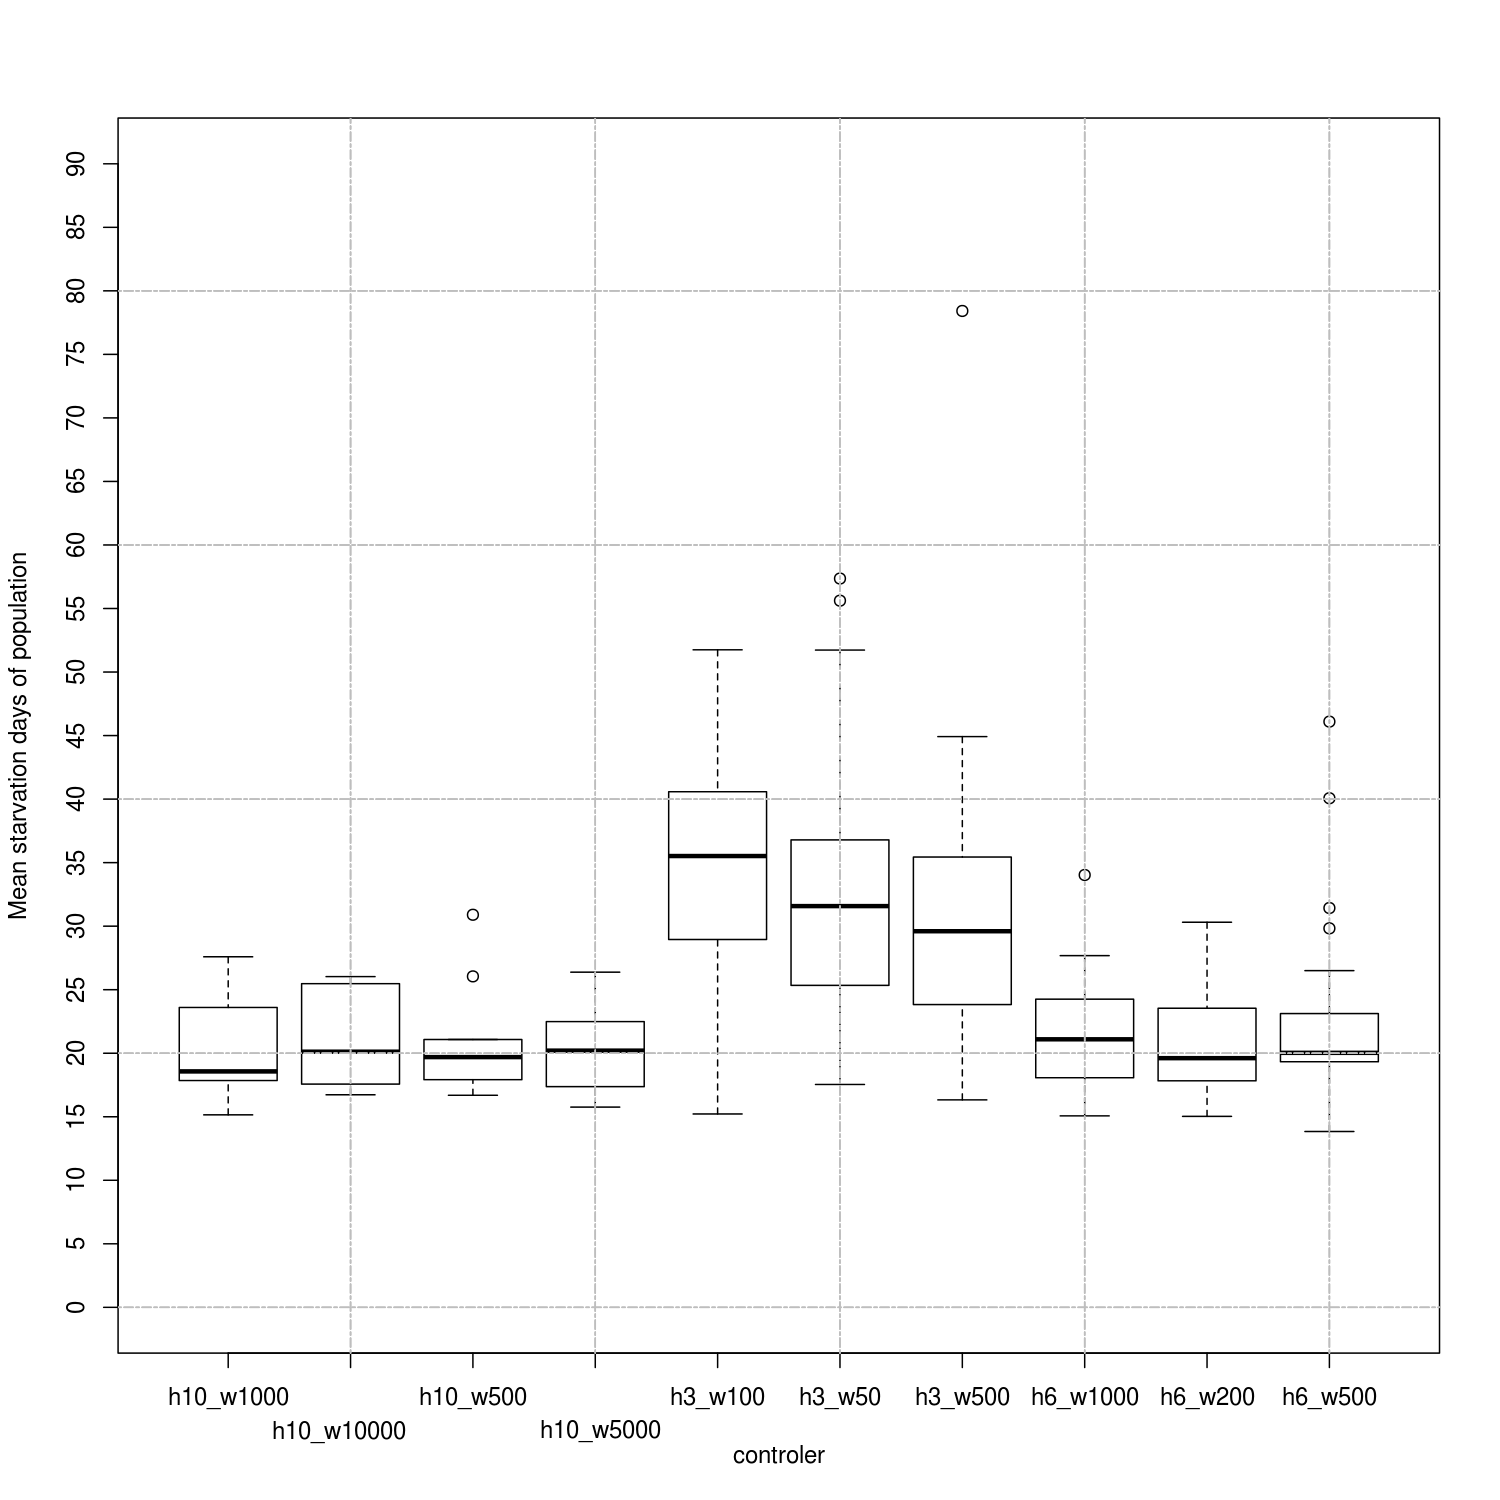
\includegraphics[height=12.2cm]{figures/expm/ecsi3_clim500}
\caption{Exploration of widths with a rainfall of 500 units.}
\label{fig:ecsi3_clim500}
\end{figure}

\begin{figure}[!htb]
\centering
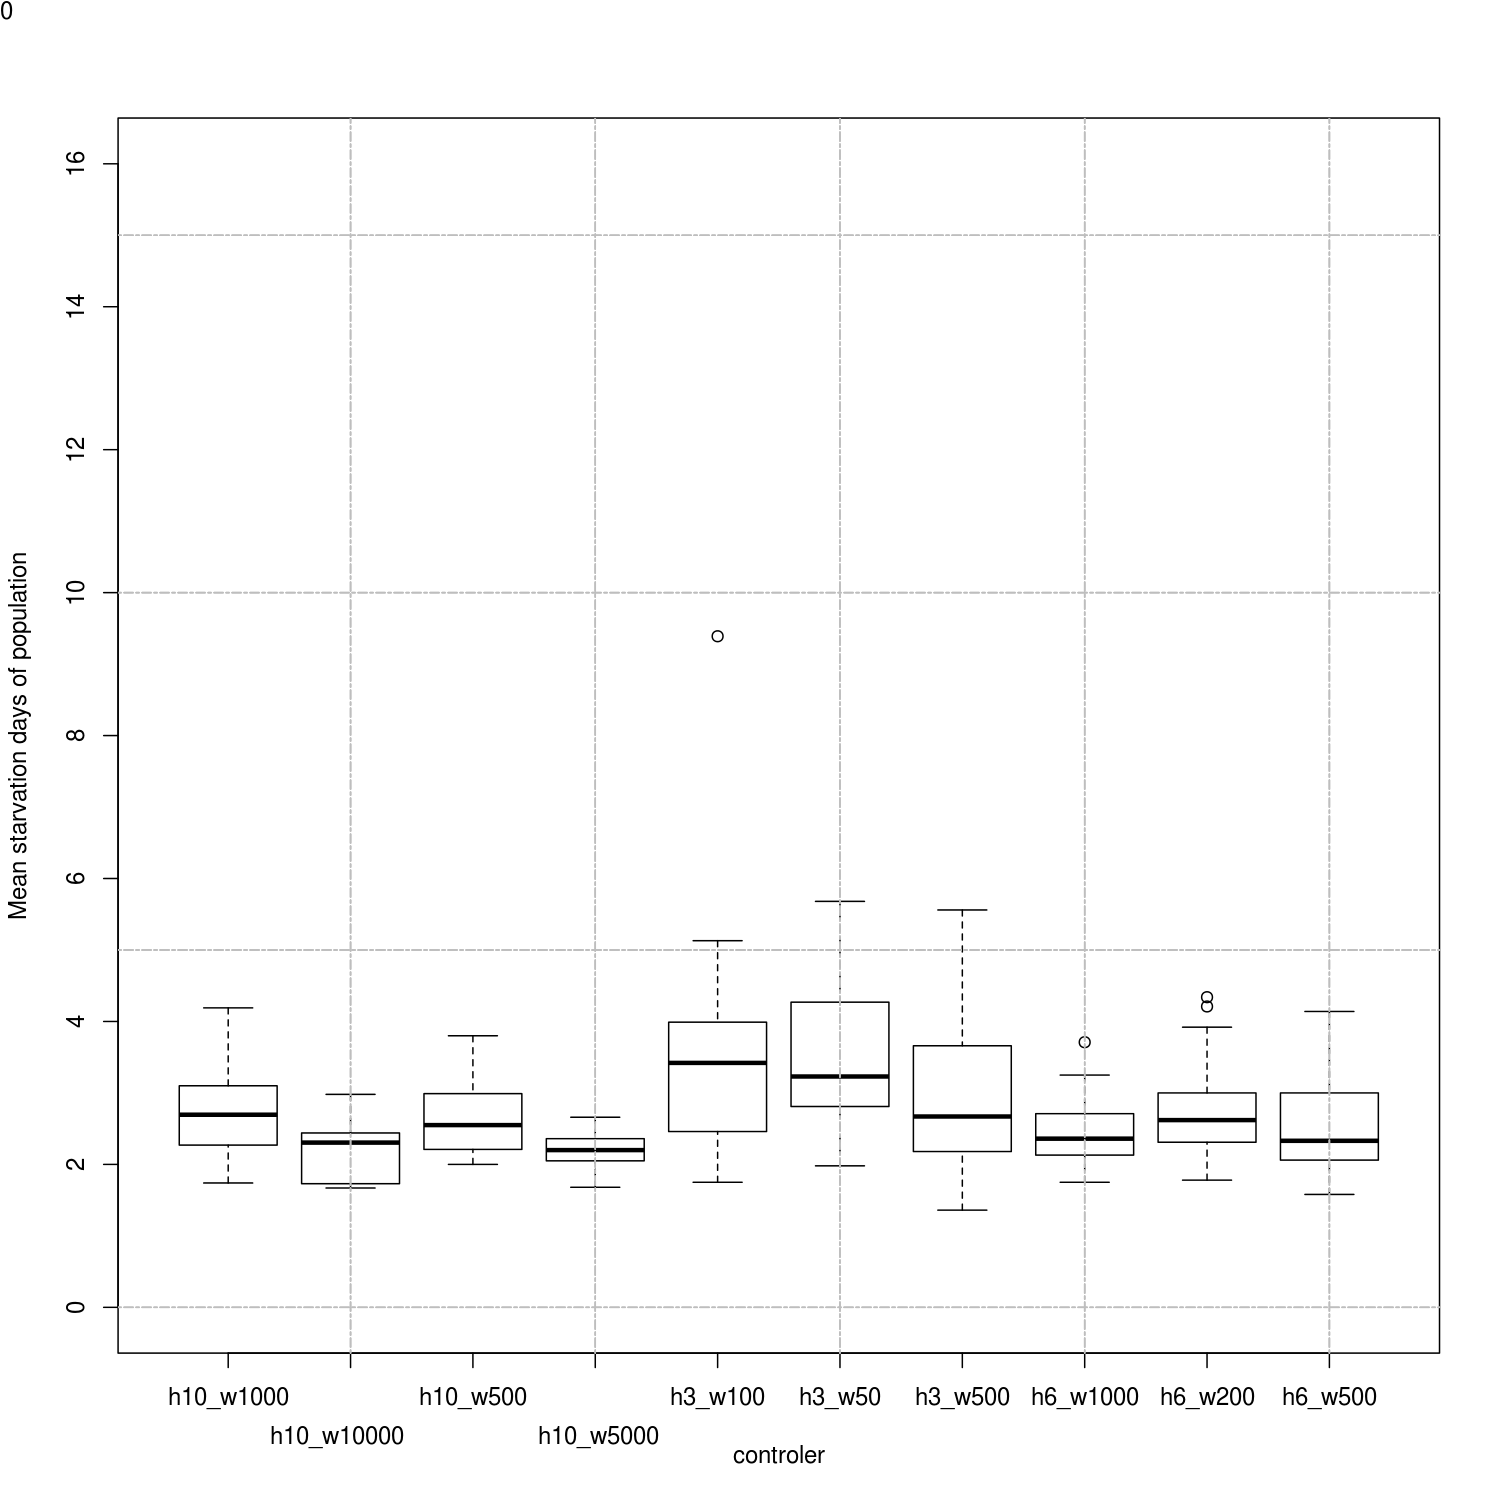
\includegraphics[height=12.2cm]{figures/expm/ecsi3_clim1500}
\caption{Exploration of widths with a rainfall of 1500 units.}
\label{fig:ecsi3_clim1500}
\end{figure}

\begin{figure}[!htb]
\centering
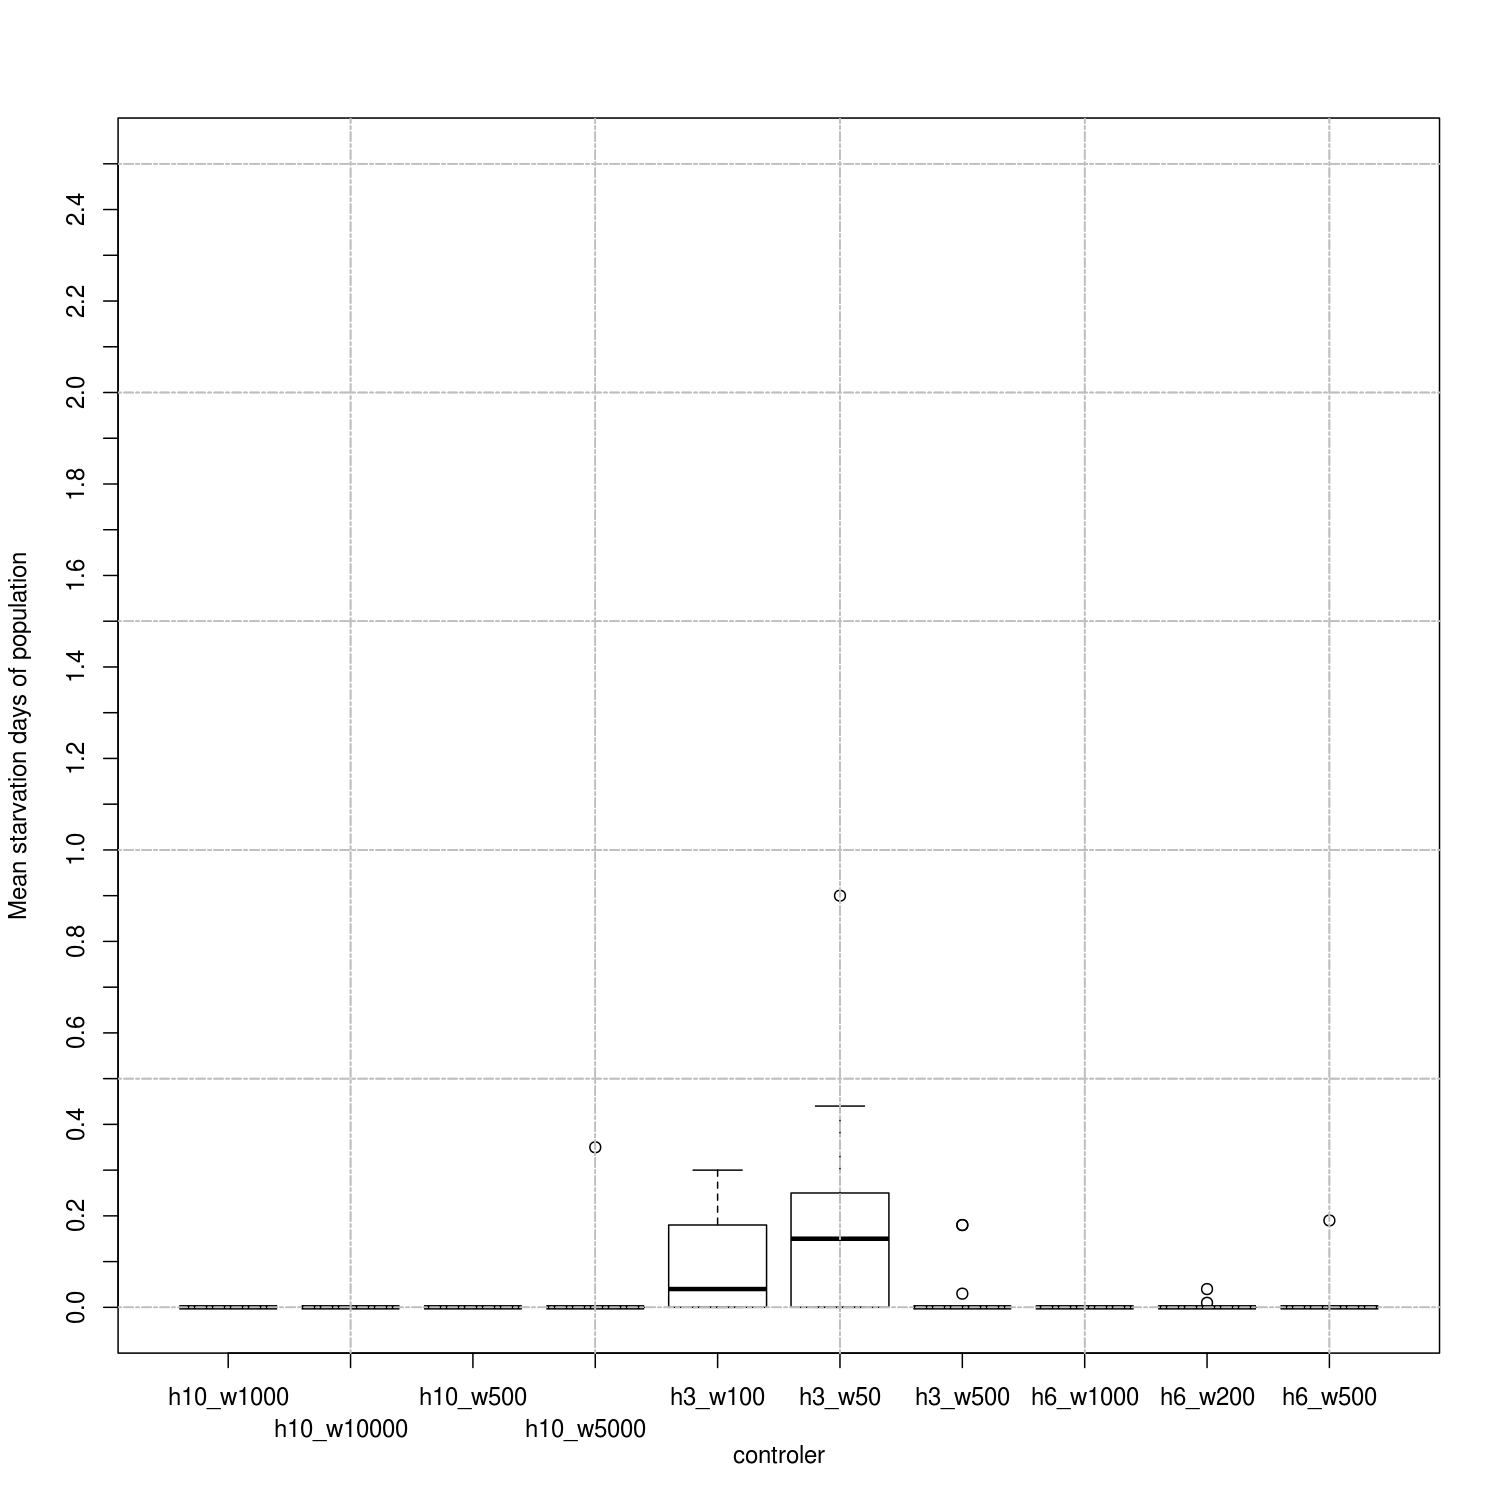
\includegraphics[height=12.2cm]{figures/expm/ecsi3_clim4000}
\caption{Exploration of widths with a rainfall of 4000 units.}
\label{fig:ecsi3_clim4000}
\end{figure}


A first approach based on the shallow evidence restates the observations from the past experiments. Horizon 6 and 10 go coupled and horizon 3 produces a lower performance of the survival skills. As rainfall increases the variability in the distribution of starvation rate decreases as decreases uncertainty and low resource states in the simulation.
It seems roughly that there is no difference when the agent uses one width or another for some given horizon. But if we look back to experiment two, they appear; it is caused by the presence of other agents who introduce uncertainty. 
When the vicinity displays greater variability in resource availability  due to the other's activities it results in having a greater range of possible states to evaluate. To explore a bigger set and filter worthy trajectories from bad ones it requires to increase the width to ensure a greater statistical significance when selecting and discarding trajectories. 
And the plots from experiment two show that agents with greater width benefit from it.

The second point, from the technical point of view, is that if with a same width with different horizons, we achieve same statistical results for the output variables in the system (e.g. starvation rate), we could extract the same conclusions. Then, the model would be statistically equivalent  under the simulated scenario and hence we could choose the configurations that imply less computational power to run cheaper and longer simulations.

%%brief conclussion:

For environments with no indirect competition the widths we have applied for each horizon do not differ very much in the survival capabilities.

% \textbf{\textit{tema resource divergence : no està esmentat, però el tenim implementat }}
% \\
% \textbf{\textit{tema divergence due to other agents in the vicinity : compto que s'ha d'esmentar al future steps}}

\subsection{Conclusions}
... brief comments, just an outline :

\begin{enumerate}

	\item summary of key evidences and conclusions from the experiments 1, 2, and 3.

	\item Una strategia basada en regles greedy pot fer escapar detalls i fer acabar dissenyant un agent poc adaptat.
	Un mateix escenari pot tenir fases on el requeriment de comportament sigui el contrari d'una a un altre; e.g. en els primers 
	dies crítics del any no et moguis; al final del any no esperis massa, move the agent often. 
	I aquest és el punt d'adaptabilitat on el rule based s'encalla.
	
	\item Els paràmetres usats per al mdp en la comparativa semblen els adients per l'objectiu. No hi ha inestabilitat, 
	i com horizon 6 es comporta bastant semblant a horizon 10 podríem dir que s'ha arribat al punt de saturació,
	més horizon no reportaria un benefici tant gran o que pogués aportar noves observacions i patrons a la 
	comparativa. Esmentant que queda prou reflexat amb aquests paràmetres que hi ha una diferència en l'us de regles versus 
	planning. ( l'experiment d'exploració de widths vs horizons ens donarà la última paraula)


	\item \textit{Una reflexio sobre agafar la AI i colocar-la en un mark diferent.}
	By the way, AI was born to emulate human performance in intelligent tasks. But it does not mean AI will give all your work done. Internal procedures in simulation are not like pure problem solving nor pure support to decision making. Many activities where AI is involved allow to AI techniques to express the power without restrictions, ``perform as best as you can'' : achieve the best accuracy on Part-Of-Speech tagging, cluster data with minimum number of false positives, produce an optimal policy for an autonomous robot, for instance. AI in social science simulation must be handled with good judgment. AI algorithms cannot be used at their fully without taking into account the cost that will represent after thousands of simulation steps. But it is more important the modelization task. AI algorithms are subjugated to the bounds(sometimes clear, sometimes fuzzy) or the features of the behaviour chosen for the agents. 

\end{enumerate}

\subsection{Future Work}

\begin{enumerate}

	\item Introduce multi-agency.
	
	\item Extrude UCT for Learning and Pattern Discovery	
	
	\item Learn social, foraging and migration rules from the stochastic explorations of UCT.
	
\end{enumerate}


%%%%%%%%%%%%%%%%%%%%%%%%%%%%%%%%%%%%%%%%%%%%%%%%%%%%%%%%%%%%%%%
\newpage
\appendix
%\chapter{Appendix}
\chapter{Reducing States of Search Tree}
\label{sec:ReduccStates}

Recall that UCT is a planning algorithm through statistical sampling. Recall that each node of the search tree corresponds to a system state and that nodes generate their node offspring to fill the next level as the result of applying a stochastic process. This would correspond to the stochastic process of change which has been produced by the effect of applying an action of the agent. States are stored in a dictionary and can be revisited if another node induces a new state that is identical to one that already has been generated in the past (Fig.~\ref{fig:reducc1}). Revisiting a state changes its weight and it guides probabilistic search and selection of actions to continue generating the range of nodes. The selection of actions affects the generation of traces that lead to final states. After executing all the amount of shots  set by the width parameter, the algorithm has performed a statistical sampling of the different states and utilities in tree leaves that end up guiding the decision.

\begin{figure}[!htb]
\centering
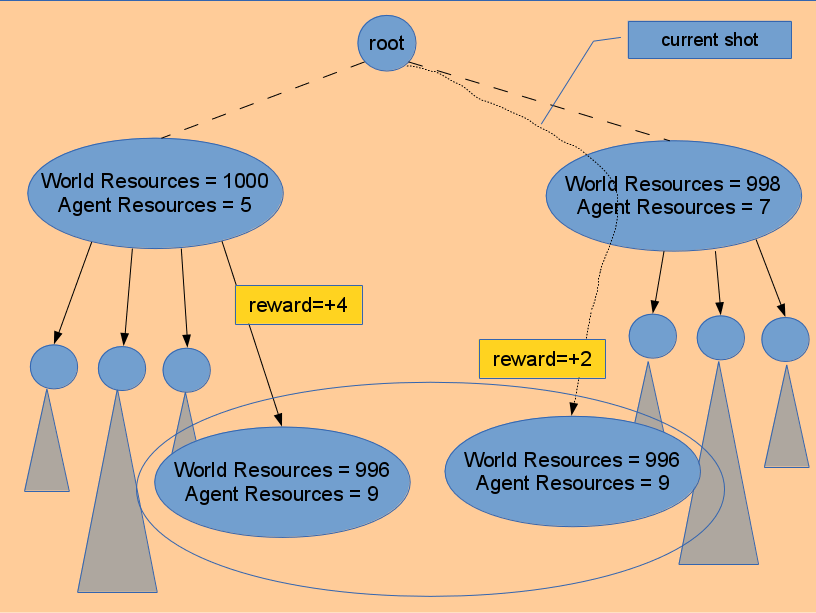
\includegraphics[height=8.2cm]{figures/diagram/reducc1}
\caption{Past states can be revisited due to stochastic effect of actions in the UCT search tree.}
\label{fig:reducc1}
\end{figure}

It is important to make relevant sampling and to crystallize significant probabilistic weights along the tree nodes, from the statistical point of view. The sampling should allow to recover an approximation of the distribution of states and utilities to filter the states which are preventable from which are desirable decisions. To visit and sample correctly traces is a need for the update factors of the underlying reinforcement learning that is done based on the sieve of the found positive and negative rewards.

In the case of the model for Hunter-gatherers, states are characterized by attributes with a wide spectrum of values. Just to mention it the amount-of-resources is the core measure of this distinctive feature. The environment of an agent is divided into sectors where the amount of resources for each one can sum up to hundreds of miles of units of biomass. If the procedure in charge of declaring two states are alike or different is based on a strict comparison of this amount, most likely, any two nodes are going to be classified as different. Taking two states where everything is the same except for the northern sector where there are 899,999 registered units in one state and the other one has an amount of 900,000, the algorithm will see both states are different and the difference is only one unit of measure of a magnitude many times over.
From the standpoint of this agent they should be considered in short-term identical because they were for survival purposes equivalent. From the point of view of the UCT algorithm, if the probability of equality between states is much lower (we trust that stochasticity after applying the action makes values match exactly by chance), part of the heuristic factors and strategies from the algorithm are not applied. The third conditional branch in code(appendix.~\ref{alg:uctAlgorithm}) will run just for a few nodes and it will hardly generate the count $N$ and $Q$ to follow the preference for rewarding promising nodes that lead to a successful trace. Then, the node will count for UCT, most of the times, as a new non visited node and the update of heuristics will be empty. The multiplicity of states emerging due to the low probability of synonymy between states will make sampled traces to be disjoint between themselves. The distribution generated is very flat because you can not make the connection between state, action and effect of the factors of Q-learning. All UCT execution will be absorbed by the branch of code that executes the basic policy, usually a random sampling. 

In order to stimulate synonymy between nodes, some changes were needed in the representation of data 
from the node states.

\begin{description}
\renewcommand{\labelitemi}{$\bullet$}
\renewcommand{\labelitemii}{$\cdot$}
\item [Value Range Reduction and Categorization] 
The idea is to encompass the same information for the decision process but in a way we reduce the range/domain of the variables. Attributes related to agent resources and environment resources are simplified.
The amount is converted to average amount of individuals sustained for a unique day by the resources. If the
original value is 400.000 units and an individual needs a mean of 2000 units to survive one day, the new value
will belong to a new reduced range and its value will be now 200 individuals per day, 200 daily rations. 
The value is reduced one step further. If an agent is composed of 4,6,10 individuals, eventually some reduced
amounts also become indistinguishable for survival. The second reduction is a categorization we have seen works for our experiments (section \ref{sec:expStateReduction}). The final assigned value to the resource attributes of the nodes is one of the categories in the table (tab.~\ref{tab:secondReductionToCategories}).

	\begin{table}[ht!]
	\centering
	\begin{tabular}{|c|c c c|}
		\hline
		CATEGORY&   &                    & \\
		\hline
		0	& 0 & $\leqslant$ rations $<$ & 2 \\
		\hline 
		1	& 2 & $\leqslant$ rations $<$ & 15 \\
		\hline
		2	& 15 & $\leqslant$ rations $<$ & 40 \\
		\hline
		3	& 40 & $\leqslant$ rations $<$ & 100 \\
		\hline
		4	& 100 & $\leqslant$ rations $<$ & $\infty$ \\
		\hline
		
	\end{tabular}
	\caption{Second reduction, categories assigned to first reduction.}
	\label{tab:secondReductionToCategories}
	\end{table}

\item [Manage Multiplicity due to Action Stochasticity] 
    Each node has actions produced depending on the information of the world state in the trace it is
    being explored. If actions are produced stochastically, same attribute sets characterizing the mensurable
    part of the state will see associated different actions sets and hence it will yield two different
    states which will end up not being equal(synonyms). We force that for a state a fixed amount of actions 
    is generated. If we allow to a state be associated to four move actions and there are eight locations
    to choose for movement, the association must be done throwing the dice and choosing four sectors
    from the eight possibilities to give four actions to the state. This increases stochasticity and
    multiplicity of states due to the combinations of taking four items from a set of eight. The solution is
    that all states open as many move actions as sectors there are, and the same for forage actions.
    And the only features involved in node matching are the relative time-step inside the trace, the resources
    of the agent, the resources of the environment, the location of the agent and the amount of accumulated days of starvation.
    
\end{description}
    
%The results of applying state reduction can be found in the section of experiments ( sect. \ref{sec:expStateReduction})


\chapter{Divergent Trajectories}
\label{sec:Divergence}
under construction...


\chapter{UCT pseudo-code}
\label{sec:uctAlgorithm}

%TODO pseudo codi de UCT tal com surt al paper de l'Hector Geffner i Bonet
\begin{algorithm}[!ht]
\caption{UCT algorithm}\label{alg:uctAlgorithm}
		\SetAlgoLined
		\BlankLine
		UCT($s$,$d$):
		{$s$ is current state; $d$ is remaining steps to depth bound; $G$ is a explicit graph, initially empty; $\pi$ is base policy; $C$ is exploration constant;}
		\BlankLine
		
		\If{d=0 or $s$ is terminal}{ 
		    \Return 0\;
		}
		\If{node($s$,$d$) not in G}
		{
		  add node ($s$,$d$) to $G$\;
		  $N$($s$,$d$) := 0\;
		  $N$($a$,$s$,$d$) := 0 for all $a \in A(s)$\;
		  $Q$($a$,$s$,$d$) := 0 for all $a \in A(s)$\;
		  Obtain sampled accumulated discounted reward $r$($\pi$, $s$, $d$)
		  by simulating base policy $\pi$ for $d$ steps starting at state $s$\;
		  \Return $r$($\pi$, $s$, $d$)\;
		}
		\If{node($s$,$d$) in G}
		{		
		$Bonus(a) = C\sqrt{2\log(N(s,d)/N(a,s,d))}$ if N($a$,$s$,$d$)$>$0,else $\infty$ for each $a \in A(s)$\;
		Select action $a$ = argmax$_{a\in A(s)}$[$Q(a, s, d) + Bonus(a)$]\;
		Sample state $s'$ with probability P$_a$($s'\mid s$)\;
		$nv$ = $r$($s$, $a$) + $\gamma$UCT($s'$ , $d \--$ 1)\;
		$N$($s$, $d$) := $N$($s$, $d$) + 1\;
		$N$($a$, $s$, $d$) := $N$($a$, $s$, $d$) + 1\;
		$Q$($a$, $s$, $d$) := $Q$($a$, $s$, $d$) + [$nv \-- Q$($a$, $s$, $d$)] / $N$($a$, $s$, $d$)\;
		\Return $nv$\;
		}		
		\caption{UCT algorithm(\cite{BonetGeffner2012})}
		\end{algorithm}



%%%%%%%%%%%%%%%%%%%%%%%%%%%%%%%%%%%%%%%%%%%%%%%%%%%%%%%%%%%%%%%


\begin{thebibliography}{2}

\bibitem{JARM2014} 
	A.L. Balbo, X. Rubio-Campillo, B. Rondelli, M. Ramírez, C. Lancelotti, A. Torrano, M. Salpeteur, 
	N. Lipovetzky, V. Reyes-García, C. Montañola, M. Madella.
	\emph{Agent-based simulation of Holocene Monsoon precipitation patterns and 
	hunter-gatherer population dynamics in semi-arid environments.} 
	Journal of Archaeological Method and Theory;vol21,issue 2.pag 426-446. Springer US 2014.
	2014


\bibitem{BonetGeffner2012}
	Hector Geffner, Blai Bonet.
	\emph{Action Selection for MDPs: Anytime AO* Versus UCT.} 
	Proceedings of the Twenty-Sixth AAAI Conference on Artificial Intelligence.	
	2012.

\end{thebibliography}
\end{document}
